\documentclass[12pt]{CSUNthesis}
%%%%%%%%%
\textheight=22cm
\def\T{\mathbb{T}}
\def\twotop#1#2{\genfrac{}{}{0pt}{}{#1}{#2}}
% % %
\def\R{\mathbb{R}}
% % % 

%%%%%%%%%
\usepackage{color}
\newcommand{\hl}[1]{\colorbox{lightgray}{#1}}
%\usepackage{tocloft}3
\usepackage{setspace}
\usepackage{amsmath}
\usepackage{amssymb}
\usepackage{graphicx}
%\usepackage{subfigure}
%\usepackage{epsfig}
\usepackage{epstopdf}
\usepackage{hyphenat}
\usepackage{setspace}
\usepackage{pdfsync}
\usepackage{tensor}
\usepackage{float}
\usepackage{subfig}
\restylefloat{table}

\setlength{\topmargin}{-0.25in}
\setlength{\textheight}{9.0in}
\setlength{\oddsidemargin}{0.5in} \setlength{\evensidemargin}{0.0in}
\setlength{\textwidth}{6.0in}

\newtheorem{example}{Example}
\newtheorem{theorem}{Theorem}
\newtheorem{proposition}{Proposition}
\newtheorem{corollary}[theorem]{Corollary}
\newtheorem{claim}[theorem]{Claim}
\newtheorem{definition}{Definition}
\newtheorem{remark}{Remark}[section]
\newtheorem{lemma}{Lemma}
\newtheorem{defn}{Definition}[section]

\newtheorem{rem}{Remark}[section]
\newenvironment{proof}[1][Proof]{\noindent\textbf{#1.} }{\newline \hspace*{\textwidth}\hspace*{-0,4cm} \rule{0.5em}{0.5em} \vspace{0,2cm}}

\renewcommand{\baselinestretch}{2}
\newcommand{\Rn}{$\mathbb{R}^n$}
\newcommand{\Rm}{$\mathbb{R}^m$}
\newcommand{\Rns}{$\mathbb{R}^n $ }
\newcommand{\Rnn}{$\mathbb{R}^{n+1}$}
\newcommand{\tb}{\textcolor{blue}}
\newcommand{\tr}{\textcolor{red}}
\newcommand{\D}{\mathrm{d}} % this defines a new command for making the d's in integrals look good
\newcommand{\limit}[3]{\underset{#1 \to #2}{\lim}  #3}  %this defines a command called limit with 3 slots
\newcommand{\manM}{$\mathcal{M}$}
\newcommand{\manMs}{$\mathcal{M} $ }
\newcommand{\Tref}{T_{\infty}}
\newcommand{\Cref}{C_{\infty}}
% Math mode friendly shortcuts
% % %
\def\T{\mathbb{T}}
\def\R{\mathbb{R}}
\def\Sbb{\mathbb{S}}
\def\e{\mathrm{e}}
\def\calF{\mathcal{F}}
\newcommand{\dydx}[2]{\frac{\partial{#1}}{\partial{#2}}}
\newcommand{\vecx}{\vec{x}}
\newcommand{\vecv}{\vec{v}}
\newcommand{\vecxi}{\vec{\xi}}
\newcommand{\bulkv}{\vec{\bar{v}}} %bulk velocity


\newenvironment{Proof}[1][Proof]{\noindent\textbf{#1.} }{\newline \hspace*{\textwidth}\hspace*{-0,4cm} \rule{0.5em}{0.5em} \vspace{0,2cm}}
%%%%%%%%%

%% ADDITIONAL COMMANDS BEGIN


%%USE TIKPICTURE
\usepackage{tikz}
\usetikzlibrary{fit}
\usetikzlibrary{shapes}
\usetikzlibrary{arrows}
\usetikzlibrary{decorations.markings}
\usetikzlibrary{positioning}

\tikzset{mylabel/.style={font=\footnotesize}}
\tikzset{mymidlabel/.style={fill=white}}
%\tikzset{mymidlabel/.style={fill=white,font=\footnotesize}}

\definecolor{mydark}{RGB}{73,68,62}%{128,129,135}
\definecolor{mymedium}{RGB}{128,129,135}%{167,170,171}
\definecolor{mylight}{RGB}{226,226,226}
\definecolor{myyellow}{RGB}{251,214,0}
\definecolor{mydarkyellow}{RGB}{255,204,13}
%%%%%%%%%%%%%%%%%%%%%%%%%%%%%

\usepackage{lmodern}
\usepackage{mathtools}
\linespread{1.0}
\usepackage[font={small,it}]{caption}
\usepackage{tabularx}
\usepackage{sidecap}
\usepackage{colortbl,xcolor}

\usepackage{algorithm,algpseudocode}


% % % Additional Commands End

%%%%%%%%%

% Set the path to graphics.
\graphicspath{{images/}}

\submitted{August}{2018}

\author{Jeffrey Limbacher}

\title{Development of Fast Methods for Evaluating the Boltzmann Collision Operator Based on Discontinuous Galerkin Discretizations in the Velocity Variable, Convolution Formulation, and Fast Fourier Transform}

\committee {Alexander Alekseenko , Ph.D.}
		   {Ali Zakeri , Ph.D.}
           {Vladislav Panferov , Ph.D.}

\abstract{tbd}

%\copyrightyear{2015}

\acknowledgement{tbd}



\begin{document}
\doublespacing

%%%%%%%%%%%%%%%%%%%%%%%%%%%%%%%%%%%%%%%%%%%%%%%%%%%%%%%%%
%%%% CHAPTER ONE
%%%%%%%%%%%%%%%%%%%%%%%%%%%%%%%%%%%%%%%%%%%%%%%%%%%%%%%%%

\chapter{Introduction}
\label{Chap1}
This thesis concerns itself with the evolution of gas flows in low density regimes. This is of particular interest to the engineering community. One example of scuh a regime is gas flows around high-altitude high-velocity objects flying through the upper atmosphere such as spacecraft and airplanes. Under such regimes, the particles impart a large amount of kinetic energy on the object causing a large transfer of heat to the object. Preventing damage to the object under these circumstances is essential. It is often difficult to replicate these conditions within a laboratory setting. This means that there is hope in the development of high fidelity solvers that can simulate the high speed gas flows around these objects to help predict the correct heating patterns. In these gas regimes, the fluid mechanical laws of Navier-Stokes and Fourier break down. In contrast, kinetic theory provide an accurate description by describing particles at the microscopic level.

Kinetic theory describes the non-equilibrium dynamics of a gas or any system comprised of a large number of particles. Kinetic equations have found applications in wide ranging applications such as rarefied gas dynamics \cite{Kremer2010} \cite{Kogan1969}, radiative transfer, and semiconductors modeling. 
The Bolzmann equation is a kinetic equation that describes gases at the molecular level at regimes where Navier-Stokes and Fourier methods fail. Analytic solutions to the Boltzmann equation have been constructed for simple geometries and special molecular potentials. However, the complexity of the equation, along with the the complexities of boundary conditions and gas-to-gas interactions that occur in engineering and physics applications, suggest that only numerical solutions are possible. However, the complexity of the equation provides a challenge in directly computing the Boltzmann equation. It is composed of a five-fold integral which must be evaluated at all points in space and velocity resulting in $\mathcal{O}(n^{11})$ computational cost where $n$ is the number of discretization points in space and velocity. This thesis primarily concerns with evaluating this integral in velocity space which results in a $\mathcal{O}(n^8)$ cost. However, this is still computationally prohibitive.

In this thesis, we explore how to speed up evaluation of the collision operator within the Boltzmann equation by using a Discontinuous-Galerkin method based on the work of \cite{Majorana2011,AlekseenkoJosyula2012,AlekseenkoJosyula2012a,GambaZhang2014}. This results in a computational complexity of $\mathcal{O}(n^8)$ with a $\mathcal{O}(n^5)$ storage requirement. In \cite{AlekseenkoNguyenWood2015}, the translational invariance was used to introduce a bilinear convolution form of the Galerkin projection of the collision operator. In the case of uniform meshes, this convolution allows us to re-write the collision operator as a convolution of multidimensional sequences. This thesis introduces a new method using the convolution theorem and Fast Fourier Transform to reduce the computational complexity of the convolution to $\mathcal{O}(n^6)$ complexity.
%%%%%%%%%%%%%%%%%%%%%%%%%%%%%%%%%%%%%%%%%%%%%%%%%%%%%%%%%
%%%% CHAPTER TWO
%%%%%%%%%%%%%%%%%%%%%%%%%%%%%%%%%%%%%%%%%%%%%%%%%%%%%%%%%

\chapter{The Boltzmann Equation}
\label{Chap2}

	The kinematic theory of gases treats gases as composed of a large number of individual molecules that, for large periods of time, flow unimpeded. As these particles move freely through space, they collide with each other. Collisions of these particles are what drive the evolution of the gas towards equilibrium.
	
	We consider a gas enclosed in a volume. A single molecule of this gas can be described with having position $\vec{x}$ and velocity $\vec{v}$ at a time $t$. For a particular time, we can describe a molecule as being within at a single point, $(\vec{x},\vec{v})$, in 6-dmensional space known as phase space. We define the distribution function of the gas as $f(t,\vec{x},\vec{v})d\vec{x}\,d\vec{v}$ gives the number of particles within the range of $\vec{x} + d\vec{x}$ with velocities $\vec{v} + d\vec{v}$. 

In 1872 Boltzmann \cite{Boltzmann1872} introduced the Boltzmann equation which describes the time evolution of the distribution $f$. In the absence of external forces and collisions of particles, then the Boltzmann equation takes the form
\begin{equation}
\label{eq:colless_boltzmann}
\dydx{}{t}f(t, \vecx, \vecv) + \vecv \cdot \nabla_x f(t, \vecx, \vecv) = 0\, .
\end{equation}
However, when the effects of collisions cannot be neglected, the right hand side must be modified. In this case, the Boltzmann equation takes the form of
\begin{equation}
\label{eq:boltzmann}
\dydx{}{t}f(t, \vecx, \vecv) + \vecv \cdot \nabla_x f(t, \vecx, \vecv) = I[f](t,\vecx,\vecv)\, \\ 
\end{equation}
Where $I[f]$ is referred to as the collision operator. The explicit form of $I[f]$ depends on the properties of the gas. To describe it explicitly, we make several assumptions. 
First, the molecules of the gas composed entirely of a single species. Second, we assume hard sphere collisions as described in section \ref{sec:bincol}.  
	
\section{Binary Collisions of Particles}
\label{sec:bincol}
	This section considers the properties of two particles on a collision path with each other as illustrated in Figure \ref{fig:binary_collision}. In all the work that follows, is is assumed that the molecules undergo elastic hard sphere collisions. 
\begin{figure}[h]
	\centering
	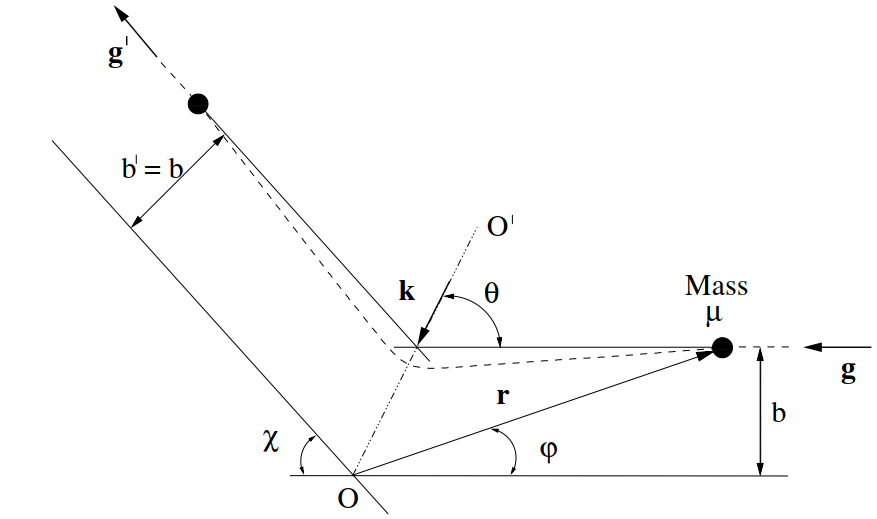
\includegraphics[scale=.5]{binary_collision}
	\caption{Kremer (2010, p. 27), Fig 1.6}
	\label{fig:binary_collision}
\end{figure}
	In Figure \ref{fig:binary_collision}, we model a particle at the point $O$. The reference frame is taken with respect to this particle. A second particle is approaching the particle at poisition $O$ symbolized by the black dot. It follows the dotted line and collides with the particle and is deflected at an angle of $\theta$ and leaves the frame.
	 Denote the pre- and post-collisional asymptotic velocities by $\vec{v}$, $\vec{v_1}$ and $\vec{v}'$, $\vec{v}_1'$ respectively. Define the relative pre- and post-collisional velocities, respectively, by 
\begin{equation*}
	\vec{g} = v_1 - v\, , \quad \vec{g}' = \vec{v}'-\vec{v}_1' \, .
\end{equation*}
$b$ denotes the offset of the centers of the molcules orthogonal to $\vec{g}$. $\varepsilon$ denotes the azimuthal angle between the two particles. 

By conservation of momentum, we have that 
\begin{equation}
\label{eq:consv_momentum}
m \vecv + m \vecv_1 = m\vecv' + m\vecv_1'\, .
\end{equation}
Equation \ref{eq:consv_momentum} yields $|g'| = |g|$. In addition, due to the hard sphere assumption, the collision is considered to be perfectly elastic, giving
\begin{equation}
\label{eq:consv_kin}
\frac{1}{2} m|\vecv| + \frac{1}{2} m|\vecv_1| = \frac{1}{2}m|\vecv'| + \frac{1}{2}m|\vecv_1'|
\end{equation}

The apsidal vector, $\vec{k}$ given by
\begin{equation*}
\vec{k} = \frac{\vec{g} - \vec{g}'}{|\vec{g} - \vec{g'}|}\, ,
\end{equation*}
bisects the angle between asymptotic relative velocities. Using this vector, we can write a relationship between the pre- and post-collisional velocities by
\begin{equation}
\label{eq:vel_relation}
\vec{v}_1' = \vec{v}_1 - \vec{k}(\vec{k} \cdot \vec{g})\, , \quad \vec{v}' = \vec{v} + \vec{k}(\vec{k} \cdot \vec{g})\, .
\end{equation}


\section{The Collision Operator}



In order to explicitly write the collision operator, we must describe the collisions within the gas. Consider a particle with velocity $\vecv_1$ at point $\vecx$. This particle will collide with $f(t,\vecx, \vecv)d\vecv_1 g \Delta t b \, db \, d\varepsilon$ particles within the ranges of $\vecv_1$ and $\vecv_1 + d\vecv_1$. Integrating this by all all possible angles $(0 \leq \varepsilon < 2 \pi)$, over all impact parameters, $(0 \leq b \leq b^*)$, and over all velocities, for all particles within the volume element $\vecx d\vecx$, we get that there are 
\begin{equation}
\label{eq:depletion}
dt \int_{\R^3} \int_0^{b^*} \int_0^{2\pi} f(t, \vecx, \vecv_1) f(t, \vecx, \vecv) b |g|\,  db \, d\varepsilon\, d\vecv_1 
\end{equation}
total collisions within the volume element that annihilate points with velocity $\vecv$. Likewise, there are collisions that create points with velocity $\vecv$. Using the results of the lasts section, points with velocity $\vecv'$ and $\vecv_1'$, impact parameter $b'=b$, and azimuthal angle $\varepsilon' = \pi + \varepsilon$ will result in particles with post-collisional velocity of $\vecv$ and $\vecv_1$. The number of such collisions is
\begin{equation}
\label{eq:restitution}
\begin{split}
&dt \int_{\R^3} \int_0^{b^*} \int_0^{2\pi} f(t, \vecx, \vecv_1') f(t, \vecx, \vecv') b' |g'|\,  db \, d\varepsilon'\, d\vecv_1 \,  \\
=&dt \int_{\R^3} \int_0^{b^*} \int_0^{2\pi} f(t, \vecx, \vecv_1') f(t, \vecx, \vecv') b |g|\,  db \, d\varepsilon\, d\vecv_1 \, .
\end{split}
\end{equation}

Subtracting (\ref{eq:depletion}) from (\ref{eq:restitution}) gives the net number of particles enter or leave the volume element $\vecv + d\vecv$; that is
\begin{equation}
\label{eq:explicit_I}
I[f](t, \vecx, \vecv) = \int_{\R^3} \int_{\R^3} (f_1' f' - f_1 f) |g|\, b\, db\, d\varepsilon\, d\vecv_1\, ,
\end{equation}
where,
\begin{equation*}
f_1' \equiv f(t, \vecx, \vecv_1')\quad f' \equiv f(t, \vecx, \vecv') \quad f_1 \equiv f(t, \vecx, \vecv_1 \quad f \equiv f(t, \vecx, \vecv)\, .
\end{equation*}
From here, we can substitute (\ref{eq:explicit_I}) into (\ref{eq:boltzmann}) to arrive to the explicit form of the Boltzmann equation,
\begin{equation}
\dydx{}{t}f(t, \vecx, \vecv) + \vecv \cdot \nabla_x f(t, \vecx, \vecv) = \int_{\R^3} \int_{\R^3} (f_1' f' - f_1 f) |g|\, b\, db\, d\varepsilon\, d\vecv_1\, .
\end{equation}
The Boltzmann equation is a non-linear integro-differential equation. The right hand side is a five dimensional integral that must be evaluated at each point in 6-dimensional space.

\section{Moments of the Distribution Function}

A gas is usually described by its macroscopic states. Kinetic theory defines these macroscopic properties in terms of distribution function $f(t,\vecx, \vecv)$. The first five moments of the gas are defined below.
\begin{align}
	n(t,\vec{x})&=\int_{\mathbb{R}^3}  f(t,\vec{x},\vec{v}) d\vec{v} &\text{- number density}  \label{eq:dens} \\
	\bar{v}_i(t,\vec{x})&=\frac{1}{n(t,\vec{x})} \int_{\mathbb{R}^3} m v_i f(t,\vec{x},\vec{v}) d\vec{v} &\text{- bulk velocity} \label{eq:bulk} \\
	T(t,\vec{x}) &= \frac{1}{3Rn(t,\vecx)}\int_{\mathbb{R}^3} m C^2 f(t,\vec{x},\vec{v}) d\vec{v} &\text{- temperature} \label{eq:temperature}
\end{align}
where $C_i=v_i-\bar{v}_i$, $C^2=C_1^2 + C_2^2 + C_3^2$, and $R$ is the specific gas constant. The number density $n(t, \vecx)$ denote the number of particles contained in our distribution. $\bulkv (t,\vecx)$ denotes that average velocity of particles within the gas. The temperature denotes the deviation form the average. 

An important property of the collision integral is that the first five moments are conservative (see \cite{Kremer2010}), that is
\begin{equation}
\label{eq:I_conservative}
\begin{split}
	\int_{\mathbb{R}^3}  I[f](t,\vec{x},\vec{v}) d\vec{v} = 0\, ,  \\
	\int_{\mathbb{R}^3} v_i I[f](t,\vec{x},\vec{v}) d\vec{v} = 0\, ,  \\
	\int_{\mathbb{R}^3} C^2 I[f](t,\vec{x},\vec{v}) d\vec{v} = 0 \, .
\end{split}
\end{equation}

\section{The Maxwellian Distribution}

If the gas is free from external influence, then the gas will approach an equilibrium. In this equilibrium, the gas distribution takes a specific shape known as the Maxwellian distribution given below.
\begin{equation}
\label{eq:maxwellian}
f_M(\vec{v},n,\vec{\bar{v}},T) = \frac{1}{\sqrt{2 \pi R T}^3} \exp\left( -\frac{ |\vec{v} - \vec{\bar{v}}|^2}{2RT} \right)
\end{equation} 
	
Note that the exact shape of the Maxwellian distribution depends on the macroscopic moments of the gas distribution, $n$, $\vec{\bar{v}}$, and $T$ given by equations (\ref{eq:dens}), (\ref{eq:bulk}), (\ref{eq:temperature}) respectively. This is illustrated in Figure \ref{fig:1d_maxwellian}. The distribution is centered around $\bulkv$. The temperature, $T$, controls the width of the distribution. $n$ determines the area under the curve. 
The Maxwellian takes a bell shaped, where $\lim_{\lvert \vec{v} \lvert \rightarrow \infty} f_M(\vec{v},n, \vec{\bar{v}}, T) = 0 $, and in fact drops off rapidly as we move away from $\vec{\bar{v}}$. This will become important later when we discretize $f_M$ (see sec \textbf{reference needed}).
\begin{figure}[h]
\centering
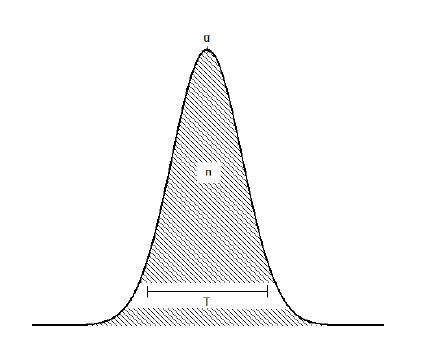
\includegraphics[scale=.5]{1D_Maxwellian}
\caption{A 1D Maxwellian distribution. }
\label{fig:1d_maxwellian}
\end{figure}

When the gas is in equilibrium, the difference between the number of particles that enter and leave a particular phase volume vanishes. In other words, 
\begin{equation*}
I[f_M](t,\vecx,\vecv) = \int_{\R^3} \int_{\R^3} (f_{M1}'f_M' - f_{M1} f_M)  g\, b\, db\, d\varepsilon\, d\vecv_1\ = 0
\end{equation*}

\section{Dimensionless Reduction}

Gas dynamic constants can vary greatly in scale. This can cause an accumulation of round-off error using floating point arithmetic when performing a large number of computations. In order to reduce the error that can be introduced by the varying scales, a dimensionless reduction is performed on the constants and equations. The dimensionless reduction aims to reduce the scale of all the variables to roughly of order one to minimize the round-off error. Note that the dimensionless reduction process can never eliminate round-off error since it is inherit to floating point arithmetic. The techniques used for dimensionless reduction vary from problem to problem. This thesis adopts the convention borrowed from Chapter 3 of [][][][].

Let $\hat{t}$, $\hat{x}$, and $\hat{v}$ denote the conventional dimensional variables. In general, all quantities bearing $\hat{\cdot}$ will represent dimensional quantities, i.e. whose numbers have units understood to have physical meaning (e.g. seconds, meters, meters per second). For example, $\hat{f}(\hat{t},\hat{x},\hat{v})$ will represent the molecular number density distribution function.

We assume some time scale $\mathbb{T}$, reference temperature $\Tref$, and some length scale $L$, which are selected with a particular application in mind. We define $\Cref = \sqrt{2R\Tref}$. In addition, we define
\begin{equation}
\label{eq:new_dimless}
t=\frac{\hat{t}}{\T},
\quad x_{i}=\frac{\hat{x}}{L},
\quad v=\frac{\hat{v}}{C_{\infty}}, 
\quad \mbox{or}
\quad \hat{t}=t\T,
\quad \hat{x}=x L,
\quad \hat{v}=vC_{\infty}\, .
\end{equation}
The dimensionless density is
\begin{equation}
f(t,x,v) = \frac{L^3 \Cref^3}{N} \hat{f}(t\mathbb{T},xL, v\Cref) = \hat{f}(\hat{t},\hat{x},\hat{v})\, ,
\end{equation}
where $N$ is total number of molecules in the gas volume $L^3$. 

With these definitions, then the relationship between the dimensionless macroparameters and the dimensional pacroparameters are now as follows. We define
\begin{equation}
\begin{split}
\label{eq:dimless_macro}
n(t,x)&:=\int_{\R^3} f(t,x,v)  dv\, ,  \\
n(t,x)\bar{u}(t,x)&:=\int_{\R^3} vf(t,x,v) dv\,  ,  \\
n(t,x)T(t,x)&:=\frac{2}{3} \int_{\R^3} (v - \bar{u})^2 f(t,x,v) dv\, , 
\end{split}
\end{equation}

From the above definitions, we get the relationships of the dimensionless and dimensional macroparameters. First note that in the discussion of follows, we have $d\hat{v} = C_{\infty}^3 dv$. Then,
\begin{equation}
\begin{split}
n(t,x) &= \int_{\R^3} f(t,x,v)  dv\, \\
&= \int_{\R^3} \frac{L^3 \Cref^3}{N} \hat{f}(\hat{t},\hat{x},\hat{v})\frac{d\hat{v}}{\Cref^3} \\
&= \frac{L^3}{N}  \int_{\R^3}  \hat{f}(\hat{t},\hat{x},\hat{v}) d\hat{v}\\
&= \frac{L^3}{N} \hat{n}(t\T,xL)\, .
\end{split}
\end{equation}
In addition,
\begin{equation}
\begin{split}
n(t,x) \bar{u}_i(t,x) &= \int_{\R^3} v_j f(t,x,v)  dv\, \\
&= \int_{\R^3} \frac{L^3 \Cref^3}{N} \frac{\hat{v}_j}{\Cref} \hat{f}(\hat{t},\hat{x},\hat{v})\frac{d\hat{v}}{\Cref^3} \\
&= \frac{L^3}{\Cref N}  \int_{\R^3} \hat{v}_j  \hat{f}(\hat{t},\hat{x},\hat{v}) d\hat{v}\\
&= \frac{L^3}{\Cref N} \hat{n}(t,x,v) \hat{\bar{u}}(\hat{t},\hat{x}) d\hat{v} \\
&= \frac{\hat{\bar{u}}_j(t,x)}{\Cref}n(t,x)\, ,
\end{split}
\end{equation}
and
\begin{equation}
\begin{split}
n(t,x)T(t,x) &= \frac{2}{3} \int_{\R^3}(v-\bar{u})^2 f(t,x,v)dv \\
&= \frac{2}{3} \int_{\R^3} \frac{L^3 \Cref^3}{N} \left( \left( \frac{\hat{v}}{\Cref} \right)^2 - \left( \frac{\hat{\bar{u}}}{\Cref} \right)^2 \right)\hat{f}(\hat{t},\hat{x},\hat{v} \frac{d\hat{v}}{\Cref^3} \\
&= \frac{2L^3}{3 \Cref^2 N} \int_{\R^3} (\hat{v} - \hat{\bar{u}})^2\hat{f}(\hat{t},\hat{x},\hat{v}) d\hat{v} \\
&= \frac{L^3}{\Tref N }\hat{n}(\hat{t},\hat{x}) T(\hat{t},\hat{x}) \\ 
&= n(t,x) \frac{\hat{T}(\hat{t},\hat{x})}{\Tref} \, .\\
\end{split}
\end{equation}
To summarize the above results,
\begin{equation}
\begin{split}
n(t,x)&=\frac{L^3 }{N} \hat{n}(\hat{t},\hat{x})\, , \nonumber  \\
\bar{u}(t,x)&=\frac{\bar{\hat{u}}(\hat{t},\hat{x})}{\Cref}\, , \nonumber \\ 
T(t,x) &= \frac{\hat{T}(\hat{t},\hat{x})}{T_{\infty}} \, . \\
\end{split}
\end{equation}

Next, the Maxwellian distribution with density $\hat{n}(\hat{t},\hat{x})$, average velocity 
$\hat{\bar{u}}_{j}(\hat{t},\hat{x})$ and temperature $\hat{T}(\hat{t},\hat{x})$ translates 
into the dimensionless Maxwellian distribution as follows:
\begin{equation}
\begin{split}
\hat{f}_{M}(\hat{t},\hat{x},\hat{u}) &= \hat{n}(2\pi R\hat{T})^{-3/2} \exp \left(- \frac{(\hat{u}-\hat{\bar{u}})^2}{2R\hat{T}}\right) \\
&= \hat{n}(2 \pi R T)^{-3/2}(\Tref / \hat{T}) ^{3/2} \exp \left(- \frac{(\hat{u}-\hat{\bar{u}})^2}{2R \Tref}\frac{\Tref}{\hat{T}}\right)\\
&= \hat{n}\pi^{-3/2} \Cref^{-3} (1/T) ^{3/2} \exp \left(- \frac{(\hat{u}-\hat{\bar{u}})^2}{T}\right)\\
&= n \frac{N}{L^3 \Cref^3} (\pi T)^{-3/2} \exp \left(- \frac{(\hat{u}-\hat{\bar{u}})^2}{T}\right)\\
&=\frac{N}{L^3 C^3_{\infty}} f_{M}(t,x,u)\, ,
\end{split}
\end{equation}
where 
\begin{equation}
f_{M}(t,x,u) :=  \frac{n}{(\pi T)^{3/2}} \exp\Bigl(-\frac{(u-\bar{u})^2}{T} \Bigr )\, . 
\end{equation}

%%%%%%%%%%%%%%%%%%%%%%%%%%%%%%%%%%%%%%%%%%%%%%%%%%%%%%%%%
%%%% CHAPTER THREE
%%%%%%%%%%%%%%%%%%%%%%%%%%%%%%%%%%%%%%%%%%%%%%%%%%%%%%%%%

\chapter{Discontinuous Galerkin Discretization in the Velocity Variable}

Discontinuous Galerkin methods is a method of discretizing equations. The following section describes the DG formulation found in~\cite{AlekseenkoJosyula2012},~\cite{AlekseenkoNguyenWood2015}.

\section{DG Discretization in Velocity Space}
We denote the points in the velocity space as $\vec{v} = (u,v,w)$. The velocity space is reduced to a rectangular parallelpiped $K=[u_L, u_R] \times [v_L,v_R] \times [w_L,w_R]$. It is assumed that outside the parallelpiped the contribution of the function to the first few moments is negligible. Depending on the parallelpiped, this will not result in large errors in terms of conservation of density and temperature. 

We partition $K$ into $N$ smaller rectangular parallelpipeds $K_j = [u_L^j, u_R^j] \times [v_L^j, v_R^j] \times [w_L^j, w_R^j]$. Each $K_j$ will contain a set of basis function, $\phi_j^i$, $i=1,\dots, s$ as described. We introduce nodes of Gauss quadratures of order $s_u$, $s_v$, and $s_w$ on each of the intervals $[u_L^j,u_R^j]$, $[v_L^j,v_R^j]$, and $[w_L^j,w_R^j]$. The nodes are denoted as
$\kappa^{u}_{p;j}$, $\dots$, $p=1,s_{u}$,
$\kappa^{v}_{q;j}$, $\dots$, $q=1,s_{v}$, and 
$\kappa^{w}_{r;j}$, $\dots$, $r=1,s_{w}$. From the nodes, the one-dimensional Lagrange basis functions are defined:
\begin{equation}
\label{eq:01}
\phi^{u}_{l;j}(u)=\prod_{{p=1,s_{u}} \atop {p\neq l}} \frac{\kappa^{u}_{p;j}-u}{\kappa^{u}_{p;j}-\kappa^{u}_{l;j}}\, ,\quad 
\phi^{v}_{m;j}(v)=\prod_{{q=1,s_{v}} \atop {q\neq m}} \frac{\kappa^{v}_{q;j}-v}{\kappa^{v}_{q;j}-\kappa^{v}_{m;j}}\, ,\quad 
\phi^{w}_{n;j}(w)=\prod_{{r=1,s_{w}} \atop {r\neq n}} \frac{\kappa^{w}_{r;j}-w}{\kappa^{w}_{r;j}-\kappa^{w}_{n;j}}\, .
\end{equation}
The three-dimensional basis function is defined as
\begin{equation}
\label{eq:01a}
\phi_{i;j}(\vec{v})=\phi^{u}_{l;j}(u)\phi^{v}_{m;j}(v)
\phi^{w}_{n;j}(w)
\end{equation} 
where $l=1, \dots , s_u$, 
$m=1,\dots ,s_v$, 
$n=1,\dots ,s_w$ and $i$ 
is the index that runs through all possible combinations of $l$, $n$, and $m$, and is computed as $i=((l-1)s_v)+(m-1)s_w)+n$.  
A useful property of the basis functions (\ref{eq:01a}) is that they vanish on all nodes except one. In addition, the quadrature nodes used are exact on polynomials of degree at most $2s_u-1$, $2s_v-1$, and $2s_w-1$. In addition, the following lemma holds,
\begin{lemma} (see also \cite{AlekseenkoJosyula2012a, HesthavenWarburtoin2007})
The following identities hold for basis functions $\phi_{i;j}(\vec{v})$:
\begin{equation}
\label{eq:lemma2.1} 
\int_{K_{j}} \phi_{p;j}(\vec{v})\phi_{q;j}(\vec{v})\, d\vec{v} = \frac{\omega_{p}\Delta\vec{v}^{j}}{8}\delta_{pq}
\qquad\mbox{and} \qquad
\int_{K_{j}} \vec{v}\phi_{p;j}(\vec{v})\phi_{q;j}(\vec{v})\, d\vec{v} 
= \frac{\omega_{p}\Delta\vec{v}^{j}}{8}\vec{v}_{p;j}\delta_{pq},
\end{equation}
where indices $l$, $n$, and $m$ of one dimensional basis functions correspond to 
the three-dimensional basis functions 
$\phi_{p;j}(\vec{v})=
\phi^{u}_{l;j}(u)\phi^{v}_{m;j}(v)\phi^{w}_{n;j}(w)$, 
and the vector $\vec{v}_{p;j}=(\kappa^{u}_{l;j},\kappa^{v}_{m;j},\kappa^{w}_{n;j})$. 
\end{lemma}
\section{Nodal-DG Velocity Discretization of the Boltzmann Equation}
We assume that on each $K_j$, the solution to the Boltzmann equation is sought of the form 
\begin{equation}
\label{eq:3.4}
f(t,\vec{x},\vec{v})|_{K_{j}} = \sum_{i=1,s} f_{i;j}(t,\vec{x})\phi_{i;j}(\vec{v})\, .
\end{equation}
We substitute equation \ref{eq:3.4} into $\ref{eq:boltzmann}$, multiply the result by test basis function, integrate over $K_j$, and apply identity (\ref{eq:lemma2.1}) to arrive to
\begin{equation}
\label{discveloblzm}
\partial_{t} f_{i;j}(t,\vec{x}) + \vec{v}_{i;j}\cdot \nabla_{x} f_{i;j}(t,\vec{x}) =
\frac{8}{\omega_{i}\Delta\vec{v}^{j}}I_{\phi_{i;j}}\, ,
\end{equation}
where $I_{\phi_{i;j}}$ is the projection of the collision operator 
on the basis function $\phi_{i;j}(\vec{v})$:
\begin{equation}
\label{eq:projcoll}
I_{\phi_{i;j}} = \int_{K_{j}}\phi_{i;j}(\vec{v}) I[f](t,\vec{x},\vec{v})\, d\vec{v}\, .
\end{equation} 

\section{Reformulation of the Galerkin Projection of the Collision Operator}
\label{sec:reform_galerkin}
Similarly to \cite{AlekseenkoJosyula2012,AlekseenkoJosyula2012a,Majorana2011}, we rewrite the 
DG projection of the collision operator $I_{\phi_{i;j}}$ in the form of a bilinear integral operator 
with a time-independent kernel. The principles of kinetic theory suggest that changes to $f(t,\vecx, \vecv)$ with respect to $\vecx$ at the distance of a few $b^*$ are negligible, see e.g., \cite{Struchtrup2005}. Specifically, using the well-known identities (see, e.g.,  \cite{Kogan1969}, Section 2.4), and applying the first principles assumption, we have 
\begin{align}
\label{eq:transfer_eq}
I_{\phi_{i;j}}&= \int_{\R^3}\int_{\R^3} f(t,\vec{x},\vec{v}) f(t,\vec{x},\vec{v}_{1})
\int_{\Sbb^2}(\phi_{i;j}(\vec{v}')-\phi_{i;j}(\vec{v})) b_{\alpha}(\theta) |g|^\alpha \, d\sigma\,
 d\vec{v}_{1}\, d\vec{v} \nonumber \\
{} & = \int_{\R^3}\int_{\R^3} f(t,\vec{x},\vec{v}) f(t,\vec{x},\vec{v}_{1})
 A(\vec{v},\vec{v}_{1};\phi_{i;j})   d\vec{v}_{1}\, d\vec{v}\, ,
\end{align}
where  
\begin{align}
\label{eq:A_definition}
A(\vec{v},\vec{v}_{1};\phi_{i;j})= |g|^\alpha \int_{\Sbb^2} (\phi_{i;j}(\vec{v}')
- \phi_{i;j}(\vec{v})) b_{\alpha}(\theta) \, d\sigma\, .
\end{align}
The kernel $A(\vec{v},\vec{v}_{1};\phi_{i;j})$ is independent of time and can be pre-computed. 
In \cite{AlekseenkoJosyula2012a} properties of a kernel closely related to $A(\vec{v},\vec{v}_{1};\phi_{i;j})$ 
are considered.
In particular, due to the local support of $\phi_{i;j}(\vec{v})$, it is anticipated that 
kernel  $A(\vec{v},\vec{v}_{1};\phi_{i;j})$ will have only $O(M^{5})$ non-zero components for each $\phi_{i;j}(\vec{v})$, 
where $M$ is the number of discrete velocity points in each velocity dimension. As a result, evaluation of  
(\ref{eq:transfer_eq}) will require $O(M^{8})$ operations for each spatial point. This number of evaluations 
is very high. However, as we will show later, it can be reduced to $O(M^6)$ operations using symmetries of
$A(\vec{v},\vec{v}_{1};\phi_{i;j})$, the convolution form of (\ref{eq:transfer_eq}) and the Fourier 
transform. 

We remark that in many numerical re-formulations of the Boltzmann equation, the collision 
operator is separated into the gain and loss terms.
This separation can be performed in (\ref{eq:transfer_eq}),
\begin{align}
\label{eq:I_split}
I_{\phi_{i;j}}&= \int_{\R^3}\int_{\R^3} f(t,\vec{x},\vec{v}) f(t,\vec{x},\vec{v}_{1})
\int_{\Sbb^2}(\phi_{i;j}(\vec{v}')-\phi_{i;j}(\vec{v})) b_{\alpha}(\theta) |g|^\alpha \, d\sigma\,
 d\vec{v}_{1}\, d\vec{v} \nonumber \\
&= \int_{\R^3}\int_{\R^3} f(t,\vec{x},\vec{v}) f(t,\vec{x},\vec{v}_{1}) (\int_{\Sbb^2}\phi_{i;j}(\vec{v}')b_{\alpha}(\theta) |g|^\alpha d\sigma\, - |g|^\alpha\int_{\Sbb^2}\phi_{i;j}(\vec{v})b_{\alpha}(\theta)  d\sigma\,)  d\vec{v}_{1}\, d\vec{v} \nonumber \\
&= \int_{\R^3}\int_{\R^3} f(t,\vec{x},\vec{v}) f(t,\vec{x},\vec{v}_{1}) (A^+(\vecv,\vecv_1;\phi_{i;j}) - |g|^\alpha \sigma_T)  d\vec{v}_{1}\, d\vec{v}
\end{align}
where
\begin{equation}
\label{eq:A_split}
A^+(\vecv,\vecv_1;\phi_{i;j}) = \int_{\Sbb^2}\phi_{i;j}(\vec{v}')b_{\alpha}(\theta) |g|^\alpha d\sigma\, , \quad \sigma_T = \int_{\Sbb^2}\phi_{i;j}(\vec{v})b_{\alpha}(\theta)  d\sigma\, .
\end{equation}
$A^+(\vecv,\vecv_1;\phi_{i;j})$ has similar properties to that of $A(\vecv,\vecv_1;\phi_{i;j})$, but
$A^+(\vecv,\vecv_1;\phi_{i;j})$ has certain properties that are better than that of $A(\vecv,\vecv_1;\phi_{i;j})$ for a Fourier transform. 
$A(\vecv,\vecv_1;\phi_{i;j})$ is grows linearly to infinity in some direction whereas $A^+(\vecv,\vecv_1;\phi_{i;j})$ does not. It can then be argued that $A^+(\vecv,\vecv_1;\phi_{i;j})$ is better suited for a Fourier transform than $A(\vecv,\vecv_1;\phi_{i;j})$. The algorithms in this paper also have straightforward extensions to the the split formulation of (\ref{eq:transfer_eq}). However, in practice, the split formulation of (\ref{eq:transfer_eq}) had significant errors in conservation.
The exact mechanism of why the non-split formulation preserves the conservation 
laws better is still not clear to the author. Some insight 
can be obtained by noticing that values of the 
collision kernel  $A(\vec{v},\vec{v}_{1};\phi_{i;j})$ span several orders of magnitude.
Small values of $A(\vec{v},\vec{v}_{1};\phi_{i;j})$ occur in
sufficiently many points so that they are important collectively. It is possible that 
when small and large values are combined during the evaluation of the gain term, the 
accuracy of the small values is lost or essentially diminished. When the loss term is subtracted from the 
gain term, cancellation occurs producing large errors. On the contrary, 
conservation 
laws are satisfied point-wise in the form (\ref{eq:transfer_eq}), 
(\ref{eq:A_definition}) up to a small number of algebraic manipulations with the basis functions 
$\phi_{i;j}(\vec{v})$. Because of these considerations, we chose to 
use the non-split form of the collision operator in simulations. 

\section{Properties of the Kernel $A(\vecv,\vecv_1;\phi_{i;j})$}
\label{sec:props_of_a} 



As stated in section \ref{sec:reform_galerkin}, $A(\vecv,\vecv_1;\phi_{i}^j)$ only contains $\mathcal{O}(M^5)$ non-zero components. This section will justify that claim by going over properties of $A(\vecv,\vecv_1;\phi_{i}^j)$. 

\begin{lemma}
\label{lem0}
Let  $A(\vecv,\vecv_1;\phi_{i}^j)$ be defined by (\ref{eq:A_definition}) with all gas particles having the same mass with the particle potentials being spherically symmetric. Then  $A(\vecv,\vecv_1;\phi_{i}^j)$ is spherically symmetric with respect to $\vecv$ and $\vecv_1$, that is
\begin{equation}
A(\vecv,\vecv_1;\phi_{i}^j) = A(\vecv_1,\vecv;\phi_{i}^j), \, \forall \vecv, \vecv_1 \in \R^3. 
\end{equation}
Also,
\begin{equation}
A(\vecv,\vecv)=0, \forall \vecv \in \R^3
\end{equation}

\end{lemma}

The next lemma establishes the shift-invariance property of $A(\vecv,\vecv_1;\phi_{i}^j)$ within the velocity space.
\begin{lemma}
\label{lem1} 
Let operator $A(\vec{v},\vec{v}_{1};\phi_{i;j})$ be defined by (\ref{eq:A_definition}). Then $\forall\xi\in \R^3$
\begin{equation*}
A(\vec{v}+\vec{\xi},\vec{v}_{1}+\vec{\xi};\phi_{i;j}(\vec{v}-\vec{\xi}))=
A(\vec{v},\vec{v}_{1};\phi_{i;j}) \, .
\end{equation*}
\end{lemma}

\proof
Consider $A(\vec{v}+\vec{\xi},\vec{v}_{1}+\vec{\xi};\phi_{i;j}(\vec{v}-\vec{\xi}))$. We clarify that these notations mean that
particle velocities $\vec{v}$ and $\vec{v}_{1}$ in (\ref{eq:A_definition}) are replaced with $\vec{v}+\vec{\xi}$ and $\vec{v}_{1}+\vec{\xi}$
correspondingly and that basis function $\phi_{i;j}(\vec{v})$ is replaced with a ``shifted'' function 
$\phi_{i;j}(\vec{v}-\vec{\xi})$. We notice that the relative speed of the molecules with velocities $\vec{v}+\vec{\xi}$ 
and $\vec{v}_{1}+\vec{\xi}$ is still $\vec{g}=\vec{v}+\vec{\xi}-(\vec{v}_{1}+\vec{\xi}_{1})=\vec{v}-\vec{v}_{1}$. 
The post-collision velocities for the pair of particles will be $\vec{v}'+\vec{\xi}$ and $\vec{v}'_{1}+\vec{\xi}$, where $\vec{v}'$ and $\vec{v}'_{1}$ are given by (\ref{eq:vel_relation}). We notice, in particular, that choices of $\theta$ and $\varepsilon$ in 
(\ref{eq:vel_relation}) are not affected by $\vec{\xi}$. The rest of the statement follows by a direct substitution:
\begin{align*}
A(\vec{v}&+\vec{\xi},\vec{v}_{1}+\vec{\xi};\phi_{i;j}(\vec{v}-\vec{\xi})) \\
&= |g|^{\alpha} \int_{\Sbb^2} \phi_{i;j}((\vec{v}'+\vec{\xi})-\vec{\xi}) b_{\alpha}(\theta)\, d\sigma\, \\
&= |g|^{\alpha} \int_{\Sbb^2} \phi_{i;j}(\vec{v}') b_{\alpha}(\theta)\, d\sigma \\
&= A(\vec{v},\vec{v}_{1};\phi_{i;j})\, . 
\end{align*}
\endproof
We remark that Lemma~{\ref{lem1}} holds for all potentials of molecular 
interaction used in rarefied gas dynamics. This property was used in 
\cite{AlekseenkoJosyula2012a} to reduce the storage requirement 
on uniform partitions.
In the case of uniform partitions with the same basis element on every cell, Information about $A(\vecv,\vecv_1;\phi_{i;j})$ need only be stored for a single cell.
Other values of $A(\vecv,\vecv_1;\phi_{i;j})$ can be restored using the shift invariance.
Strictly speaking, one requires an infinite partition of the entire velocity space to recover all points. However, assuming that the support of the solution is well contained within a finite domain, the shift invariance property can be used successfully. 






\section{Rewriting the Collision Operator in the Form of a Convolution}
It was shown in~\cite{AlekseenkoNguyenWood2015} that the Galerkin projection of the collision operator can be reformulated in terms of a convolution. This work is recalled in this section. 
We select a partition cell $K_c$ and designate this cell as a generating cell. 
Similarly, the basis functions $\phi_{i;c}(\vec{v})$ on $K_c$ are designated as the generating basis functions. 
Basis functions $\phi_{i;j}(\vec{v})$ on other cells can be obtained using a shift in the velocity variable, namely $\phi_{i;j} (\vec{v})=\phi_{i;c} (\vec{v}+\vec{\xi_{j}})$ where $ \vec{\xi}_{j} \in \mathbb{R}^3$ is the vector that connects the center of $K_j$ to the center of $K_c$.

According to  Lemma~{\ref{lem1}}, operator $A(\vec{v},\vec{v}_1,\phi_{i;j})$ is invariant with respect to translations. Therefore
\begin{align}
\label{eq3.1}
I_{\phi_{i;j}} &= \int_{\R^3}\int_{\R^3} f(t,\vec{x},\vec{v})f(t,\vec{x},\vec{v}_{1})A(\vec{v}+\vec{\xi_{j}},\vec{v}_1+\vec{\xi_{j}}; \phi_{i;j}(\vec{u} - \vec{\xi_{j}})) \, d\vec{v}_{1} d\vec{v} \notag\\
 &= \int_{\R^3}\int_{\R^3} f(t,\vec{x},\vec{v})f(t,\vec{x},\vec{v}_{1})A(\vec{v}+\vec{\xi^{j}},\vec{v}_{1}+\vec{\xi_{j}}; \phi_{i;c}(\vec{u})) \, d\vec{v} d\vec{v_{1}} \, .
\end{align}
Performing the substitutions $\vec{\hat{v}} = \vec{v}+\vec{\xi_{j}} $ and $ \vec{\hat{v}}_1 = \vec{v}_{1}+\vec{\xi_{j}}$ in (\ref{eq3.1}), we have
\begin{equation*}
I_{\phi_{i;j}} = \int_{\R^3}\int_{\R^3} f(t,\vec{x},\vec{\hat{v}}-\vec{\xi_{j}}) f(t,\vec{x},\vec{\hat{v}}_1-\vec{\xi_{j}}) A(\vec{\hat{v}},\vec{\hat{v}}_{1};\phi_{i;c}(\vec{u})) \, d\vec{\hat{v}} d\vec{\hat{v}}_1 \, .
\end{equation*}
We then introduce a bilinear convolution operator, $i=1,\ldots,s$
\begin{equation}
\label{eq:continuous_convolution}
I_i(\vec{\xi}) = \int_{\R^3}\int_{\R^3} f(t,\vec{x},\vec{v}-\vec{\xi})f(t,\vec{x},\vec{v}_{1}-\vec{\xi})A(\vec{v},\vec{v}_{1}; \phi_{i;c}) \, d\vec{v} d\vec{v}_{1} \, ,
\end{equation}
and notice that $I_{\phi_{i;j}}$ can be obtained from (\ref{eq:continuous_convolution}) as
$I_{\phi_{i;j}}=I_i(\vec{\xi}_j)$. In the following, we will refer to (\ref{eq:continuous_convolution}) 
as the convolution form of the Galerkin projection of the collision integral.

\section{Discretization of the Collision Integral}
In order to calculate (\ref{eq:continuous_convolution}), we replace the three-dimensional integrals with the Gauss quadratures associated with then nodal-DG discretization, (\ref{eq:01a}). 
As is discussed above, we are only interested in 
computing convolution (\ref{eq:continuous_convolution}) at vectors 
$\vec{\xi}=\vec{\xi}_{j}$ that connect centers of the velocity cells $K_j$ to the 
center of the velocity cell $K_c$, the support of $\phi_{i;c}(\vec{v})$. Since the 
same nodal points are used on all velocity cells, shifts $\vec{\xi}_{j}$ 
translate nodal points in one cell to nodal points 
in another cell. As a result, the quadrature sums to evaluate convolution (\ref{eq:continuous_convolution})
use values of the unknown $f(t,\vec{x},\vec{v})$ at the nodal points
only. In fact, the shift in the velocity variable 
$\vec{v}_{i;l}-\vec{\xi}_{j}$ will correspond 
to a shift in the three dimensional index of the velocity cell 
which we will write formally as $l-j$, 
producing the velocity node $\vec{v}_{i;l-j}(\vec{v})$. The exact expression 
for the shift $l-j$ will be made clear later by considering the cell indices in 
each velocity dimension. The index $i$ of the node within the cell is not 
affected in this process. 

We can write the discrete form of (\ref{eq:continuous_convolution}) as 
\begin{equation}
\label{eq:I_dist}
I_{i;j}:=I_{i}(\vec{\xi}_{j}) = \sum_{i',i''=1}^s  \sum_{j'=1}^{M^3} \sum_{j''=1}^{M^3} f_{i';j'-j} f_{i'';j''-j} A_{i',i'';j',j'';i} 
\end{equation}
where $f_{i';j'-j}=f(t,\vec{x},\vec{v}_{i';j'-j})$, 
$A_{i',i'';j',j'';i}=A(\vec{v}_{i';j'},\vec{v}_{i'';j''}; \phi_{i;c})$ and the three dimensional 
indices $i'$ and $i''$ run over the velocity nodes within a single velocity cell 
and indices $j'$ and $j''$ run over all velocity cells. We note that for some index 
shifts $j'-j$, the resulting cells are outside of the velocity domain. 
In \cite{AlekseenkoJosyula2012a} the values outside of the domain 
were substituted with zeros. In cases when the support of the solution 
was well contained within the computational domain, this assumption did not lead to 
large numerical errors. 

We note that in order to calculate (\ref{eq:I_dist}), it would require $O(M^9)$ operations to calculate it, $O(M^6)$ at one velocity node for $O(M^3)$ velocity nodes. However, recall the property stated in section \ref{sec:reform_galerkin} that $A$ only has $O(M^5)$ components bringing down the total cost of computing (\ref{eq:I_dist}) down to $O(M^8)$ operations. However, we wish to reduce this further. It turns out that the Discrete Fourier Transform has properties that allow us to bring down the cost of computing (\ref{eq:I_dist}) from $O(M^8)$ to $O(M^6)$. The DFT and its properties are discussed in the next section.

\section{The Micro-Macro Decomposition}
The form of the collision integral can be reformulated for the purpose of numerical implementation. During simulations, it was observed that the ability of numerical simulations to conserve mass, momentum, and energy is strongly affected by the form of the discrete collision integral. 

One such reformulation is the micro-macro decomposition [{\bf ??}] which considers the solution has the sum of the target Maxwellian distribution and the deviation from the Maxwellian, i.e.,
\begin{equation}
\label{eq:decomp}
f(t,\vecx,\vecv) = f_M(t, \vecx, \vecv) + \Delta f(t,\vecx,\vecv)\, ,
\end{equation}
where $f_M(t,\vecx,\vecv)$ takes the form (\ref{eq:maxwellian}) with the same temperature, bulk velocity, and temperature as $f(t,\vecx,\vecv)$. This form was applied in \cite{AlekseenkoJosyula2012} in order to improve conservation properties of the scheme when the solution is near continuum. The numerical implementation used for the FFT convolution also used this decomposition. We substitute (\ref{eq:decomp}) into (\ref{eq:transfer_eq}) to obtain an alternative form of the collision integral:
\begin{align}
\label{eq:I_decomp_continuous}
I_{\phi_{i;j}}&= \int_{\R^3}\int_{\R^3} f(t,\vec{x},\vec{v}) f(t,\vec{x},\vec{v}_{1})
 A(\vec{v},\vec{v}_{1};\phi_{i;j})   d\vec{v}_{1}\, d\vec{v}\, \nonumber \\
 &=\int_{\R^3}\int_{\R^3} [f_{M}(t,\vec{x},\vec{v}) \Delta f(t,\vec{x},\vec{v}_{1})
 +\Delta f(t,\vec{x},\vec{v}) f_{M}(t,\vec{x},\vec{v}_{1})\nonumber \\
 &\hspace*{10mm}{}+ \Delta f(t,\vec{x},\vec{v}) \Delta f(t,\vec{x},\vec{v}_{1})]
 A(\vec{v},\vec{v}_{1};\phi_{i;j})   d\vec{v}_{1}\, d\vec{v}\, . 
\end{align}
where we used that $I[f_M](t,\vecx,\vecv)=0$. It was found that this form of the operator provided much better numerical results. Thus the numerical results in the rest of this work use (\ref{eq:I_decomp_continuous}) for all the calculations. 

%%%%%%%%%%%%%%%%%%%%%%%%%%%%%%%%%%%%%%%%%%%%%%%%%%%%%%%%%
%%%% CHAPTER FOUR
%%%%%%%%%%%%%%%%%%%%%%%%%%%%%%%%%%%%%%%%%%%%%%%%%%%%%%%%%

\chapter{The Discrete Fourier Transform}

The goal is to compute (\ref{eq:I_dist}) faster than $O(M^8)$. We note that (\ref{eq:I_dist}) is similar to a discrete convolution form (which will be defined later). The Discrete Fourier Transform (DFT) can be used to speed up the computations of convolutions using the \textit{Convolution Theorem}. In particular, it is used to speed up circular convolutions. In order to apply the DFT to our problem, we must first assume a periodic extension of the discrete form of $f$. This section discusses the background of the Discrete Fourier Transform, convolution theorem, and periodic continuation needed to quickly compute (\ref{eq:I_dist}) 

\section{The One-Dimensional Discrete Fourier Transform and its Properties}

The Discrete Fourier Transform is the discrete analog of the Fourier transform. It is a tool often used describe the relationship between the time and frequency representation of discrete signals \cite{Nussbaumer1982}. 
\begin{definition}
Let $\{x_n\}_{n=0}^{N-1}$ be a sequence of $N$ complex numbers. The DFT is defined as
\begin{equation}
\label{eq:dft_1d}
\calF[x]_{k} =  \sum_{l=0}^{N-1} W^{lk} x_l, \qquad  
\mbox{where}\quad 
W=\e^{-\imath 2\pi/N}\, .
\end{equation}
\end{definition}

\subsection{Properties of the DFT}

Many properties of the DFT are a natural consequence of its defintion. In this subsection, we review the properties of the DFT that will be important for applying the DFT to \ref{eq:I_dist}. First, the DFT is invertible.

\begin{definition}
Let $\{\calF [x]_k\}_{k=0}^{N-1}$ be a sequence of $N$ complex numbers such that it is the DFT of the complex valued sequence $\{x_l\}_{l=0}^{N-1}$. Then the inverse DFT is defined as
\begin{equation}
\label{eq:idft_1d}
x_{l} = \frac{1}{N} \sum_{k=0}^{N-1} W^{-lk} \calF[x]_{k} \, .
\end{equation}
\end{definition}

We can see that definition of the inverse will give back the original sequence. If we have a sequence $\{x_l\}_{l=0}^{N-1}$, then note that if we take the inverse of $\calF[x]_k$

\begin{align*}
\calF^{-1}[\calF[x]]_l &= \frac{1}{N} \sum_{k=0}^{N-1}W^{-lk}(\sum_{j=0}^{N-1} W^{kj} x_j) \\
 &= \frac{1}{N} \sum_{k=0}^{N-1} \sum_{j=0}^{N-1} W^{-lk} W^{kj} x_j \\
 &= \frac{1}{N} \sum_{j=0}^{N-1}  x_j (\sum_{k=0}^{N-1} W^{(j-l)k}) \\
 &= N \frac{1}{N} x_l = x_l
\end{align*}
where the last step used that if $l \not = j$ then $\sum_{k=0}^{N-1} W^{(j-l)k} = 0$ and for $l=j$ we have that $\sum_{k=0}^{N-1} W^{(j-l)k} = \sum_{k=0}^{N-1} 1 = N$. Thus the definition given above returns the original sequence. To see this:
\begin{align*}
\calF[z]_k &= \sum_{l=0}^{N-1} W^{kn} \sum_{n=0}^{N-1} x_{n}y_{l-n} \\
&= \sum_{n=0}^{N-1} x_{n} ( \sum_{l=0}^{N-1} W^{kn}y_{l-n})
\end{align*}

The DFT is linear. That is, if we have two complex sequences $\{x_n\}_{n=0}^{N-1}$ and $\{y_n\}_{n=0}^{N-1}$, then 
\begin{equation}
\label{eq:dft_lin}
\calF[x+y]_k = \calF[x]_k + \calF[y]_k\, .
\end{equation}
This property will be used in order to apply the DFT to discrete convolution form of the collision integral.

The last property we need is the shift property. This says that if $\{y_n\}$ is a periodic sequence created by shifting $\{x_n\}$ by $l$, that is $\{y_n\} = \{x_{n-l}\}$, then
\begin{equation}
\label{eq:shift_prop}
\calF[y]_k = W^{kl}\calF[x]_k\, .
\end{equation}
To see this
\begin{align*}
\calF[y]_k &= \sum_{n=0}^{N-1} W^{kn} y_n \\
&= \sum_{n=0}^{N-1} W^{kn} x_{n-l} \\
&= \sum_{n=0}^{N-1}  W^{k(n-l)} x_{n-l} \\
&= W^{kl} \sum_{n=0}^{N-1} W^{k(n-l)}x_{n-l} \\
&= W^{kl} \calF[x]_k\, .
\end{align*}
\subsection{The Convolution Theorem}
Another important result is the convolution theorem. The result is stated and proved here. First we start with a definition.
\begin{definition}
Let $x_{n}$ and $y_{n}$ be periodic sequences with period $N$. An $N$-point circular 
convolution of $x_{n}$ and $y_{n}$ is defined as (see, e.g., \cite{Nussbaumer1982})
\begin{equation}
\label{eq:cirlconv}
z_{l}=\sum_{n=0}^{N-1} x_{n}y_{l-n}\, ,  \quad l=1,\dots,N-1 \, .
\end{equation} 
\end{definition}
We are now ready to state the convolution theorem.
\begin{theorem}
Let $\{x_n\}$ and $\{y_n\}$ be $N$-periodic sequences. Let $z_l$ denote the circular convolution given by (\ref{eq:cirlconv}). Then
\begin{equation}
\label{eq:dft_circ_conv}
\calF[z]_{k}=\calF[x]_{k}\calF[y]_{k}\, .
\end{equation}
\end{theorem}
\begin{proof}
This can be proven with a straight forward use of the definition of the DFT and the circular convolution,
\begin{align*}
\calF[z]_k &= \sum_{l=0}^{N-1} W^{kl} \left( \sum_{n=0}^{N-1} x_n y_{l-n} \right) \\
&= \sum_{n=0}^{N-1} x_n \left( \sum_{l=0}^{N-1} W^{kl} y_{l-n} \right) \\
&= \sum_{n=0}^{N-1} x_n W^{kn} \calF[y]_k \\
&= \calF[y]_k \left( \sum_{n=0}^{N-1} x_n W^{kn}\right)\\
&= \calF[y]_k \calF[x]_k \, ,
\end{align*}
where we used the shift property (\ref{eq:shift_prop}) of the DFT, e.g. $\sum_{l=0}^{N-1} W^{kl} y_{l-n} = W^{kl} \calF[y]_k$
\end{proof}
After calculating $\calF[z]_k$ using (\ref{eq:dft_circ_conv}), the sequence $\{z_n\}_{n=0}^{N-1}$ can be retrieved via application of the inverse DFT, (\ref{eq:idft_1d}), e.g. $\calF^{-1}[\calF[z]]_n = z_n$. 


The convolution theorem seemingly gives no computational gain. Straightforward computation of the DFT and inverse DFT will take $O(N^2)$ complex operations. Computation of (\ref{eq:cirlconv}) also takes $O(N^2)$ operations without needing to perform any complex multiplications if both $\{x_n\}$ and $\{y_n\}$ are real. However, the complexity of calculating (\ref{eq:dft_1d}) can be reduced by an algorithm known as the Fast Fourier Transform (FFT) which can calculate both the forward and inverse DFT in $O(N \log N)$ operations.

\section{Circular Convolution as Linear Convolution}
\subsection{Linear Convolutions and Circular Convolutions}
{\textbf rewrite} The DFT can be used to calculate circular convolutions quickly. However, while (\ref{eq:I_dist}) has a form similar to the definition of a circular convolution, we note that it is not a circular convolution. In the discussion that follows (\ref{eq:I_dist}), we mention that for an $f_{i;j}$ with $j \leq 0$ or $j > M$, we set $f_{i;j}=0$. If (\ref{eq:I_dist}) was truly a circular convolution, then we must assume that $f_{i;j}=f_{i;j+M}$ for any $j \leq 0$ or $f_{i;j}=f_{i;k-M}$ for any $j > M$. 

Formally, (\ref{eq:I_dist}) is a linear convolution. However, this section will show that there are deep connections between linear convolutions and circular convolutions. Indeed, there are conditions where they can be considered equivalent. This allows us to treat (\ref{eq:I_dist}) as circular convolution and use the convolution theorem of the DFT and the speed up provided by the Fast Fourier Transform algorithm to calculate (\ref{eq:I_dist}) quickly. The discussion here is inspired by Oppenheim, Shafter and Buck Digital signal processing (add citation).

\subsection{Linear Convolution of Two Finite-Length sequences}
\label{sec:lin_conv_fin_seq}
For the sake of ease of notation for later discussions, we introduce a linear convolution for infinite sequences. 
\begin{definition}
Let $\{x_n\}_{n=-\infty}^{\infty}$, $\{y_n\}_{n=-\infty}^{\infty} \subset \mathbb{C}$ be sequences of (possibly complex) numbers. Then a linear convolution is defined as 
\begin{equation}
\label{eq:lin_conv}
z_{l}=\sum_{n=-\infty}^{\infty} x_{n}y_{l-n}\, , l \in \mathbb{N}
\end{equation}
\end{definition}


If the sequences are finite sequences of length $L$, then we may set $x_n=0$ and $y_n=0$ if $n<0$ or $n \geq L$. In that case, the above definition readily extends to finite sequences.

Suppose we have two sequences $\{x_n\}_{n=-\infty}^{\infty}$,$\{y_n\}_{n=-\infty}^{\infty} $ 
such that $ x_n \ = 0$ for $n<0$ and $n\geq L$ and $ y_n \ = 0$ for $n<0$ and $n \geq P$, and let $z_l$ be the result of performing a linear convolution between these two sequences. Note that $x_n y_{l-n}=0$ for $l < 0$ and $l > L + P - 2$. In other words, $z_l \not = 0$ for $0 \leq l \leq L + P - 2$. If $\{x_n\}$ and $\{y_n\}$ are finite sequences, then $z_l$ is also a finite sequence of maximum length $L+P-1$. In this, using finite sequences, we can rewrite the sum (\ref{eq:lin_conv}) as 

\begin{equation}
\label{eq:finite_lin_conv}
z_l = \sum_{n=\max(0,l-(P-1))}^{\min(L-1,l)} x_n y_{l-n}
\end{equation}

\subsection{Linear Convolution as Circular Convolution}
\label{sec:lin_circ_eq}
	Due to the similarity of the definition of the linear convolution (\ref{eq:lin_conv}) and the circular convolution (\ref{eq:cirlconv}), there are conditions in which linear convolutions and circular convolutions are equivalent. The linear convolution involves multiplying a sequence by a index-reversed and shifted version of the other, then summing the products, i.e. $x_n y_{l-n}$ where $y_n$ is reversed and shifted. The circular convolution also reverses and shifts, but in particular, the finite sequences of $\tilde{x}_n$ and $\tilde{y}$ are periodic. However, if we extend the sequences $\tilde{x}_n$ and $\tilde{y}_n$ in the appropriate manner, we can eliminate the difference between the linear convolution and circular convolution of sequences. 
	

	We start with a motivating example. Let's examine the case where $x_n=1$ for $n=0,\dots,4$ and $y_n=1$ for $n=0,\dots,4$. The linear convolution would be calculated as
	
\begin{equation}
\label{eq:lin_conv_example}
z_l = \sum_{n=-\infty}^{\infty } x_n y_{l-n} = \begin{cases}
x_0 y_0 &= 1, \quad l=0\\
x_0 y_1 + x_1 y_0 &= 2, \quad l=1\\
& \vdots \\ 
x_0y_4 + \dots + x_4 y_0 &= 5, \quad l=4 \\
& \vdots \\
x_4y_0 &= 1, \quad l= 8 \\
0 &\text{ otherwise}
\end{cases}
\end{equation}
	The linear convolution gives a triangular sequence, $z_l = \min(l+1,9-l)$ for $l=0, \dots, 8$. However, if we were to directly do a circular convolution, we would simply get $\tilde{z}_l = 5$ for $ l=0, \dots, 4$. 
	However, let $\{ \tilde{x}_n \}$ and $\{\tilde{y}\}$ be periodic sequences of period 9 such that $\tilde{x}_n = x_n$, $\tilde{y}_n = y_n$ for $n=0, \dots, 4$ and $\tilde{x}_n=\tilde{y}=0$ otherwise. Let $\tilde{z}_n$ denote the sequence generated by the circular convolution of $\tilde{x}_n$ and $\tilde{y}_n$. Then note that (\ref{eq:lin_conv_example}) still holds for $\tilde{z}_n$. 

	The insight is that we can \textit{pad} the sequences with zeroes such that the zeros remove any extra terms added by the circular convolution. Let $z_n$ denote the result of linear convolution of $\{x_n\}$ and $\{y_n\}$. Suppose we have periodic sequences $\{\tilde{x}_n\}$, $\{\tilde{y}_n\}$ such that $\tilde{x}_n = x_n$ for $0 \leq n < L$ and $\tilde{x}_n = 0$ for $L \leq n \leq L+P-2$, and $\tilde{y}_n = y_n$ for $0 \leq n < P$ and $\tilde{y}_n = 0$ for $L \leq n \leq L+P-2$. Set $N=L+P-2$.
Let $\tilde{z}$ denote the sequence generated by taking the $N$-point circular convolution of $\tilde{x}$ and $\tilde{y}$. Then we have that $\tilde{z}_n = z_n$. 

To see this, note that for $l=0$, we have that $N$-point convolution becomes  $\sum_{n=0}^{L+P-2} \tilde{x}_n \tilde{y}_{l-n} = \tilde{x}_0 \tilde{y}_0$ since $\tilde{x}_1, \dots \tilde{x}_{L-1}$ is going to be multiplied against $\tilde{y}_{L+P-2}, \dots, \tilde{y}_{L+P-2-(L-2)}$ $=\tilde{y}_{P}$ which are all zero. Then for $l=1$, we must have that $\tilde{z}_l = \sum_{n=0}^{L+P-2} \tilde{x}_n \tilde{y}_{l-n} = \tilde{x}_0 \tilde{y}_1 + \tilde{x}_1 \tilde{y}_0$ which agrees with equation (\ref{eq:finite_lin_conv}). Thus we have shown how to recover the linear convolution using the circular convolution.

	Now that we have shown that we can indeed recover a linear convolution using a circular convolution with zero padding, we can now apply the convolution theorem to linear convolutions.  To see this, if we set $N > L+P-2$, so if we take an $N$-point circular convolution of $\{x_n\}$ and $\{y_n\}$, (or equivalently $\{\tilde{x}_n\}$ and $\{\tilde{y}_n\}$, then we have that
\begin{align*}
\calF[z]_k = \calF[x]_k \calF[y]_k\, ,
\end{align*}
where $\calF$ denotes the $N$-point DFT. In particular, with the correct zero padding, we can apply the DFT to (\ref{eq:I_dist}) with no error.
\subsection{Circular Convolution as Linear Convolution with Aliasing.}

We saw that we can find an equivalence between the linear convolution and the circular convolution by zero padding the finite sequences $\{ x_n\}$ and $\{y_n\}$. However, in certain cases, zero-padding may not be possible. In this section we explore what happens when we are unable to zero-pad the sequences.

Suppose $\{x_n\}_{n=0}^{L-1}$ and $\{y_n\}_{n=0}^{P-1}$ For simplicity, let $L \geq P$. If we take an $L$-point DFT of $\{x_n\}$ or $\{y_n\}$ then we can perfectly reconstruct both $\{x_n\}$ and $\{y_n\}$ given $\{ \calF[x]_k \}$ and $\{ \calF[y]_k \}$. Now suppose $z_l$ is the linear convolution of $\{x_n\}$ and $\{y_n\}$, so $z_l$ is of length $L+P-1$. 
If we attempt to calculate $\calF[z]_k$ using the convolution theorem, we expect it to be incorrect because an $L$-point DFT would be insufficient. 
Suppose we attempt to calculate $\calF[z]_k$ by using the convolution theorem, i.e. 
\begin{equation}
\label{eq:aliasing}
\calF[z]_k^* = \calF[x]_k \calF[y]_k \, . 
\end{equation}
Then we can expect that in general $\calF^{-1}[\calF[z]^*]_l \not = z_l$. We refer to this as \textit{aliasing error}. This occurs because by trying to calculate the linear convolution using the covolution theorem, we are implicitly using a circular convolution in (\ref{eq:aliasing}). As discussed in section \ref{sec:lin_circ_eq}, taking an $L$-point DFT is insufficient to capture the correct values for $z_l$. 

\section{The One-Dimensional Fast Fourier Transform}
The Fast-Fourier Transform (FFT) is an algorithm that reduces the complexity of calculating the DFT. As can be seen from the definition of the DFT, (\ref{eq:dft_1d}), calculating the DFT of an $N$-point sequence takes $\mathcal{O}(N^2)$ operations. However, the FFT reduces the algorithmic complexity of the DFT to $\mathcal{O}(N \log N)$. This is a significant increase. In addition, due to the convolution theorem (\ref{eq:dft_circ_conv}), we can now calculate circular convolutions in $\mathcal{O}(N \log N)$ as opposed to $\mathcal{O}(N^2)$ operations.

This section will discuss the details of the FFT algorithm and how it achieves its lower computational complexity. Let $\{x_n\}_{n=0}^{N-1}$ be a sequence and $\calF[x]_k$ be its DFT. By definition, we have
\begin{equation}
\label{eq:dft_2}
\calF[x]_k = \sum_{n=0}^{n-1} x_n W^{nk}
\end{equation}
Suppose $N=N_1 N_2$ with $N_1,$ $N_2 \in \mathbb{N}$. We can redefine the indices $n$ and $k$ with 
\begin{align}
\label{eq:m1k1}
m &= N_1 n_1 + n_1 , & m_1 , k_1 = 0, \dots, N_1-1 \\
\label{eq:m2k2}
k &= N_2 k_1 + k_2 , & k_2 , m_2 = 0, \dots, N_2-1 \, .
\end{align}
Substitution of (\ref{eq:m1k1}) and (\ref{eq:m2k2}) into (\ref{eq:dft_2}) gives 
\begin{equation}
\label{eq:dft_composite}
\calF[x]_{N_2k_1 + k_2} = \sum_{n_1=0}^{N_1-1} W^{N_2n_1k_1}W^{n_1k_2} \sum_{n_2=0}^{N_2-1} x_{N_1 n_2+ n_1} W^{N_1 n_2k_2} \, .
\end{equation}
We define
\begin{equation*}
W_1 := e^{-i 2 \pi / N_1} = W^{N_2}\, \quad W_2 = e^{-i 2 \pi / N_2} = W^{N_1}\, ,
\end{equation*}
and rewrite (\ref{eq:dft_composite}) as
\begin{equation}
\label{eq:first_step}
\calF[x]_{N_2k_1 + k_2} = \sum_{n_1=0}^{N_1-1} W_1^{n_1k_1}W^{n_1k_2} \sum_{n_2=0}^{N_2-1} x_{N_1n_2+n_1} W_2^{n_2k_2} \, .
\end{equation}
This shows that the DFT of size $N_1N_2$ can be viewed as a three step process. First, we calculate $N_1$ DFTs which correspond to the $N_1$ values of $n_1$. We denote these by 
\begin{equation}
\calF[x]_{n_1,k_2} = \sum_{n_2=0}^{N_2-1} x_{N_1n_2+n_1} W_2^{n_2k_2} \, .
\end{equation}
Second, $\calF[x]_{n_1,k_2}$ is multiplied against the \textit{twiddle factors} $W^{n_1k_2}$. Third, $\calF[x]_k$ is then obtained by calculating $N_2$ DFTs of the $N_1$ DFTs on the $N_2$ input sequences of $\calF[x]_{n_1,k_2}W^{n_1k_2}$, with
\begin{equation}
\label{eq:third_step}
\calF{x}_{N_2k_1+k_2} = \sum_{n_1=0}^{N_1-1}\calF[x]_{n_1,k_2}W^{n_1 k_2}W_1^{n_1k_1} \, .
\end{equation}

If we were to calculate the DFT an $N=N_1N_2$ sequence directly, then we would require $N_1^2N_2^2$ multiplications. However, using the algorithm corresponding to (\ref{eq:first_step}) and (\ref{eq:third_step}), then computations are broken down into $N_1$ DFTs of $N_2$ terms and $N_2$ DFTs of $N_1$ terms plus $N_1N_2$ multiplications for the twiddle factors. Thus the number of multiplications for calculating the DFT of the $N_1N_2$ points reduces to
\begin{equation*}
N_1N_2^2 + N_2N_1^2 + N_1N_2 = N_1N_2(N_1+N_2+1)
\end{equation*}
number of multiplications which is less than the original $N_1^2N_2^2$ multiplications.

While this does not result in the claimed $\mathcal{O}(N \log N)$ multiplications, the algorithm can be used recursively when $N$ is highly composite. We can decompose the original $N$-point DFT into DFTs of length $N_1$ and $N_2$ which can then be further decomposed such that each can be computed using the FFT algorithm. This feature motivates the application of the FFT to DFT lengths which are the power of an integer, and in most cases $N$ is chosen to be a power of 2 \cite{Nussbaumer1982}.

We can now consider the DFT of an $N$-point sequence $\{x_n\}_{n=0}^{N-1}$ with $N=2^t$. In this case, we can do the first stage of the FFT using $N_1 = 2$ and $N_2 = 2^{t-1}$. This results in splitting the original input sequence $x_n$ into two $(N/2)$-point sequences, $x_{2n}$ and $x_{2n+1}$ which correspond to the even and odd indices of the original $x_n$ respectively.
%%%%%%%%%%%%%%%%%%%%%%%%%%%%%%%%%%%%%%%%%%%%%%%%%%%%%%%%%
%%%% CHAPTER FIVE
%%%%%%%%%%%%%%%%%%%%%%%%%%%%%%%%%%%%%%%%%%%%%%%%%%%%%%%%%

\chapter{Discretization of the Collision Integral and Fast Evaluation of Discrete Convolution}


\section{Formulas for Computing the DFT of the Collision Integral Copy and Pasted}
To derive the formula for computing the collision operator we rewrite (\ref{eq:I_dist}) as
\begin{equation}
\label{I+_distq1}
I_{i;j_{u},j_{v},j_{w}}= \sum_{i',i''=1}^s I_{i,i',i'';j_{u},j_{v},j_{w}} \, ,
\end{equation}
where 
\begin{equation*}
I_{i,i',i'';j_{u},j_{v},j_{w}}=  \sum_{j_u',j_v',j_w'=0}^{M-1} \sum_{j_u'',j_v'',j_w''=0}^{M-1} f_{i';j'_{u}-j_{u},j'_{v}-j_{v},j'_{w}-j_{w}} f_{i'';j''_{u}-j_{u},j''_{v}-j_{v},j''_{w}-j_{w}} A_{i',i'';j'_{u},j'_{v},j'_{w},j''_u,j''_{v},j''_{w};i}\, .
\end{equation*}
In view of (\ref{I+_distq1}), we can focus on evaluation of $I_{i,i',i'';j_{u},j_{v},j_{w}}$. 
To simplify the notations in the discussion below, we drop the $i$, $i'$, and $i''$ subscripts from 
$I_{i,i',i'';j_{u},j_{v},j_{w}}$, $f_{i';j'_{u},j'_{v},j'_{w}}$, 
$A_{i',i'';j'_{u},j'_{v},j'_{w},j''_u,j''_{v},j''_{w};i}$, and  $\calF[I_{i,i',i''}]_{k_{u},k_{v},k_{w}}$ 
and write $I_{j_u,j_v,j_w}$, $f_{j'_{u},j'_{v},j'_{w}}$, 
$A_{j'_{u},j'_{v},j'_{w},j''_u,j''_{v},j''_{w}}$, and $\calF[I]_{k_{u},k_{v},k_{w}}$, respectively. 
In particular, we have
\begin{equation}
\label{I_all_index}
I_{j_u,j_v,j_w}=  \sum_{j_u',j_v',j_w'=0}^{M-1} \sum_{j_u'',j_v'',j_w''=0}^{M-1}f_{j'_{u}-j_{u},j'_{v}-j_{v},j'_{w}-j_{w}} f_{j''_{u}-j_{u},j''_{v}-j_{v},j''_{w}-j_{w}} A_{j'_{u},j'_{v},j'_{w},j''_u,j''_{v},j''_{w}}\, .
\end{equation}
As is seen from definition (\ref{mdft_def}), the multi-dimensional DFT results from applying the one-dimensional DFT along each dimension of the sequence for every fixed value of indices in the other dimensions (see e.g., \cite{Nussbaumer1982}).

We fix indices $j_v$ and $j_w$  in equation (\ref{I_all_index}) and apply the one-dimensional DFT in the remaining index $j_u$. Using linearity of the DFT and reordering the sums, we have 
\begin{equation*}
\calF[I_{j_v,j_w}]_{k_u} = \sum_{j_v',j'_w=0}^{M-1} \sum_{j_v'',j''_{w}=0}^{M-1}  \calF[\hat{I}_{j_v,j_v',j_v'',j_w,j_w',j_w''}]_{k_u}\, ,
\end{equation*}
where 
\begin{equation*}
\calF[\hat{I}_{j_v,j_v',j_v'',j_w,j_w',j_w''}]_{k_u} = 
\sum_{j_u=0}^{M-1}  W^{ k_u j_u} \hat{I}_{j_u;j_v,j_v',j_v'',j_w,j_w',j_w''} 
\end{equation*}
\begin{equation*}
\hat{I}_{j_u;j_v,j_v',j_v'',j_w,j_w',j_w''} = \sum_{j_u''=0}^{M-1} \sum_{j_u'=0}^{M-1} f_{j'_{u}-j_{u},j'_{v}-j_{v},j'_{w}-j_{w}} f_{j''_{u}-j_{u},j''_{v}-j_{v},j''_{w}-j_{w}} A_{j'_{u},j'_{v},j'_{w},j''_u,j''_{v},j''_{w}}\, .
\end{equation*}
Once again, for purposes of calculating the one-dimensional discrete Fourier transform along dimension $j_u$, we need only consider the transform of $\hat{I}_{j_u,j_v,j_v',j_v'',j_w,j_w',j_w''}$. 
By similar argument as before, we fix and drop indices $j_v$, $j_v'$, $j_v''$, $j_w$, $j_w'$, and $j_w''$ in the latter formula and write 
\begin{align}
\hat{I}_{j_u} &= \sum_{j_u''=0}^{M-1} \sum_{j_u'=0}^{M-1} f_{j'_{u}-j_{u}} f_{j''_{u}-j_{u},} A_{j'_{u},j''_u} \label{I_onedim_u} \\
\calF[\hat{I}]_{k_u} &= \sum_{j_u=0}^{M-1} \sum_{j_u''=0}^{M-1} \sum_{j_u'=0}^{M-1} W^{k_u j_u} f_{j'_{u}-j_{u}} f_{j''_{u}-j_{u},} A_{j'_{u},j''_u}\, . \label{FI_onedim_u}
\end{align}
We note that evaluating $\calF[\hat{I}]_{k_u}$ directly would require $O(M^3)$ operations.
However, taking into consideration the discussion in the last section, expression in the right side of (\ref{I_onedim_u}) can be considered as a circular convolution, having a form similar to (\ref{cirlconv}). This motivates us to explore properties of the DFT and rewrite (\ref{FI_onedim_u}) in a form suitable for numerical computation. This is accomplished in the following lemma.

\begin{lemma}
\label{lemma_dft}
Let $\{ f_j\}_{j=0}^{M-1}$ be a $M$ periodic sequence and $\{A_{ij}\}_{ij}$ be a two index sequence that is $M$ periodic in both its indices. Let $\{\hat{I}_j\}_{j=0}^{M-1}$ be a new sequence defined by 
\begin{equation}
\label{I_onedim}
\hat{I}_{j} =  \sum_{j'=0}^{M-1} \sum_{j''=0}^{M-1} f_{j'-j}f_{j''-j} A_{j',j''} 
\end{equation}
Let $\calF[\hat{I}]_k$ be the DFT of $\hat{I}_j$, then  
\begin{equation}
\label{onedfconv}
\calF[\hat{I}]_k = M \sum_{l=0}^{M-1} \calF^{-1}[f]_{k-l} \calF^{-1}[f]_{l} \calF[A]_{k-l,l}
\end{equation}
\end{lemma}

\begin{proof}
Applying the one-dimensional DFT to $\hat{I}_j$, we have
\begin{equation}
\label{FI_u_index}
\calF[\hat{I}]_k = \sum^{M-1}_{j_u=0} \sum^{M-1}_{j'=0} \sum^{M-1}_{j''=0} W^{k j } f_{j'-j}f_{j''-j}A_{j',j''}
\end{equation}
We define $\calF[A_{j'}]_{l}$ to be the one-dimensional DFT of $A_{j',j''}$ in the second index, i.e.,
\begin{align*}
%\label{ondim_FAdef}
\calF[A_{j'}]_{l} = \sum_{j''=0}^{M-1} W^{ j'' l} A_{j',j''}\, ,
\end{align*}
and rewrite $A_{j',j''}$ as
\begin{align}
\label{one_dim_FA}
A_{j',j''}= \frac{1}{M} \sum_{l=0}^{M-1} W^{ -j'' l} \calF[A_{j'}]_{l}\, .
\end{align}
Substituting (\ref{one_dim_FA}) into (\ref{FI_u_index}), we have
\begin{align}
\label{original}
\calF [\hat{I}]_k &= \frac{1}{M} \sum_{j=0}^{M-1} \sum_{j'=0}^{M-1} \sum_{j''=0}^{M-1} W^{jk} f_{j'-j}f_{j''-j}
\left( \sum_{l=0}^{N-1} W^{-j'' l} \calF[A_{j'}]_{l} \right)  \nonumber \\
&= \frac{1}{M} \sum_{l=0}^{M-1} \sum_{j=0}^{M-1} \sum_{j'=0}^{M-1} \sum_{j''=0}^{M-1} W^{jk} f_{j'-j}f_{j''-j} W^{-j'' l } \calF[A_{j'}]_{l} 
\end{align}
Consider the sum that runs over index $j''$. Assuming that indices $l$, $j$, and $j'$ are held constant, we split the sum into two parts.
\begin{align}
\label{j''_split}
&\sum_{j''=0}^{M-1} W^{jk} f_{j'-j}f_{j''-j} W^{-j'' l } \calF[A_{j'}]_{l}  \nonumber \\
=&\sum_{j''=0}^{j-1} W^{jk} f_{j'-j}f_{j''-j} W^{-j'' l } \calF[A_{j'}]_{l} + \sum_{j''=j}^{M-1} W^{jk} f_{j'-j}f_{j''-j} W^{-j'' l } \calF[A_{j'}]_{l} \, .
\end{align}

Notice $j''-j < 0$ in the first sum. Using the periodicity of $f_{j}$ the summation index can be redefined so that only values $f_{j''-j}$ with positive $j''-j$ appear in the sum. Indeed, we assume that $j'' < j$ and notice that $f_{j''-j}=f_{j''-j+M}$ since $f_{j}$ is $M$ periodic. We also have $W^{M}=1$, so $W^{j'' l } = W^{j''l+Ml} = W^{(j''+M)l}$. 
Introducing $\hat{j}''=j''+M$, we observe 
\begin{align*}
\sum_{j''=0}^{j-1} W^{jk} f_{j'-j}f_{j''-j} W^{-j'' l } \calF[A_{j'}]_{l} &
=\sum_{j''=0}^{j-1} W^{jk} f_{j'-j}f_{j''-j+M} W^{(-j''+M) l } \calF[A_{j'}]_{l} \\
&=\sum_{\hat{j}''=M}^{M-1+j} W^{jk} f_{j'-j}f_{\hat{j}''-j} W^{-\hat{j}'' l } \calF[A_{j'}]_{l}\, . 
\end{align*}
Combining the last formula with (\ref{j''_split}) we have 
\begin{align}
\label{j''_split2}
\sum_{j''=0}^{M-1} W^{jk} f_{j'-j}f_{j''-j} W^{-j'' l } \calF[A_{j'}]_{l} 
&= \sum_{j''=j}^{M-1+j} W^{jk} f_{j'-j}f_{j''-j} W^{-j'' l } \calF[A_{j'}]_{l} \, .
\end{align}
Introducing a substitution of index $u''=j''-j$ we rewrite the right side of  (\ref{j''_split2}) as follows 
\begin{align*}
\sum_{j''=0}^{M-1} W^{jk} f_{j'-j}f_{j''-j} W^{-j'' l } \calF[A_{j'}]_{l} 
= \sum_{u''=0}^{M-1} W^{jk} f_{j'-j}f_{u''} W^{(-u''-j) l } \calF[A_{j'}]_{l}\, .
\end{align*}
Going back to (\ref{original}), we replace the inside sum with the last expression to have
\begin{align}
\label{original_u''}
\frac{1}{M} \sum_{l=0}^{M-1} &\sum_{j=0}^{M-1} \sum_{j'=0}^{M-1} \sum_{u''=0}^{M-1} W^{jk} f_{j'-j}f_{u''} W^{(-u''-j) l } \calF[A_{j'}]_{l} \nonumber \\
&= \frac{1}{M} \sum_{l=0}^{M-1} \sum_{j'=0}^{M-1} \sum_{u''=0}^{M-1} W^{-u'' l }f_{u''} \left( \sum_{j=0}^{M-1} W^{j(k-l)} f_{j'-j}  \calF[A_{j'}]_{l}  \right)\, .
\end{align}

Now we focus on the term within the parentheses in (\ref{original_u''}). Splitting the sum and using periodicity, we obtain
\begin{align}
\sum_{j=0}^{M-1}& W^{j(k-l)} f_{j'-j} \calF[A_{j'}]_{l} \\
&=\sum_{j=0}^{j'} W^{j(k-l)} f_{j'-j} \calF[A_{j'}]_{l} + \sum_{j=j'+1}^{M-1} W^{j(k-l)} f_{j'-j} \calF[A_{j'}]_{l}  \nonumber \\
&=\sum_{j=0}^{j'} W^{j(k-l)} f_{j'-j} \calF[A_{j'}]_{l} + \sum_{j=j'+1}^{M-1} W^{(j-M)(k-l)} f_{j'-j+M} \calF[A_{j'}]_{l}  \nonumber \\
&=\sum_{j=0}^{j'} W^{j(k-l)} f_{j'-j} \calF[A_{j'}]_{l} + \sum_{\hat{j}=j'-M+1}^{-1} W^{\hat{j}(k-l)} f_{j'-\hat{j}} \calF[A_{j'}]_{l}  \nonumber  \\
&=\sum_{j=j'-M+1}^{j'} W^{j(k-l)} f_{j'-j} \calF[A_{j'}]_{l} 
= \sum_{u'=0}^{M-1} W^{(j'-u')(k-l)} f_{u'} \calF[A_{j'}]_{l}\, .
\end{align}
Here $u'=j'-j$. 
Substituting this result into (\ref{original_u''}) and regrouping sums, we yield
\begin{align}
\label{grouped}
\frac{1}{M} \sum_{l=0}^{M-1} &\sum_{j'=0}^{M-1} \sum_{u''=0}^{M-1} W^{-u'' l }f_{u''} \left( \sum_{j=0}^{M-1} W^{j(k-l)} f_{j'-j}  \calF[A_{j'}]_{l}  \right) \nonumber \\
&= \frac{1}{M} \sum_{l=0}^{M-1} \sum_{j'=0}^{M-1} \sum_{u''=0}^{M-1} W^{-u'' l}f_{u''} \left(\sum_{u'=0}^{M-1} W^{(j'-u')(k-l)} f_{u'} \calF[A_{j'}]_{l} \right) \nonumber \\
&= M\sum_{l=0}^{M-1} \left( \frac{1}{M} \sum_{u'=0}^{M-1} W^{-u'(k-l)} f_{u'}  \right) \left( \frac{1}{M} \sum_{u''=0}^{M-1} W^{-u'' l} f_{u''} \right) \left(  \sum_{j'=0}^{M-1} W^{j'(k-l)} \calF[A_{j'}]_{l} \right).
\end{align}
The terms in the parentheses in (\ref{grouped}) are just the definitions of the DFT. Thus we can write the equation as
\begin{align*}
\calF [\hat{I}]_k = M \sum_{l=0}^{M-1} \calF^{-1}[f]_{k-l} \calF^{-1}[f]_l \calF[A]_{k-l,l} \, .
\end{align*}
\end{proof}

Lemma~\ref{lemma_dft} allows us to compute (\ref{FI_onedim_u}) in $O(M^2)$ operations. Indeed, it takes 
$O(M \log M)$ operations to compute $\calF^{-1}[f]_{k_{u}}$ using a fast Fourier transform and it takes 
$O(M^2)$ operations to compute discrete convolution in the frequency space (\ref{onedfconv}). To extend this result to $\calF[I]_{k_{u},k_{v},k_{w}}$, it is sufficient to repeat the approach for indices $j_{v}$ and $j_{w}$ focusing on one dimension at a time. The following theorem summarizes the result. 

\begin{theorem}
\label{thm3.1}
Let $f_{j_{u},j_{v},j_{w}}$ be a three-index sequence that is periodic in each index with period $M$ and let $A_{j'_{u},j'_{v},j'_{w},j''_{u},j''_{v},j''_{w}}$ be a $M$-periodic six-dimensional tensor. The multi-dimensional discrete Fourier transform of equation (\ref{I_all_index}) can be represented as
\begin{equation}
\label{FI_formula}
\calF [I]_{k_{u},k_{v},k_{w}} = M^3 \sum_{l_{u},l_{v},l_{w}=0}^{M-1} \calF^{-1}[f]_{k_{u}-l_{u},k_{v}-l_{v},k_{w}-l_{w}} \calF^{-1}[f]_{l_{u},l_{v},l_{w}} \calF[A]_{k_{u}-l_{u},k_{v}-l_{v},k_{w}-l_{w},l_{u},l_{w},l_{w}}
\end{equation}
\end{theorem}

\begin{proof}
We apply the one dimensional discrete Fourier transform along $j_u$ in equation (\ref{I_all_index}) and apply Lemma {\ref{lemma_dft}}:
\begin{align}
\label{lemma_once}
\calF[I_{j_v,j_w}]_{k_{u}}&= \sum_{j_v',j_w'=0}^{M-1} \sum_{j_v'',j_w''=0}^{M-1} \left(\sum_{j_u=0}^{M-1} \sum_{j_u'=0}^{M-1} \sum_{j_u''=0}^{M-1} W^{j_u k} f_{j_u'-j_u,j_v'-j_v,j_w'-j_w} f_{j_u''-j_u,j_v''-j_v,j_w''-j_w} A_{j'_{u},j'_{v},j'_{w},j''_u,j''_{v},j''_{w}}\right) \nonumber \\ 
&= M\sum_{j_v',j_w'=0}^{M-1} \sum_{j_v'',j_w''=0}^{M-1} \sum_{l_{u}=0}^{M-1} \calF^{-1}[f_{j_v'-j_v,j_w'-j_w}]_{k_{u}-l_{u}} \calF^{-1}[f_{j_v''-j_v,j_w''-j_w}]_{l_u} \calF[A_{j'_{v},j'_{w},j''_{v},j''_{w}}]_{k_{u}-l_{u},l_{u}} \nonumber \\ 
&= M\sum_{l_u=0}^{M-1} \sum_{j_w'=0}^{M-1} \sum_{j_w''=0}^{M-1} \nonumber \\
& \hspace{10mm} 
\left( \sum_{j_v'=0}^{M-1} \sum_{j_v''=0}^{M-1}   \calF^{-1}[f_{j_v'-j_v,j_w'-j_w}]_{k_{u}-l_{u}} \calF^{-1}[f_{j_v''-j_v,j_w''-j_w}]_{l_{u}} \calF[A_{j'_{v},j'_{w},j''_{v},j''_{w}}]_{k_{u}-l_{u},l_{u}} \right) .
\end{align}

We now focus on the terms inside the parentheses. We fix the indices $j_w$, $j_w'$, $j_w''$, $k_{u}$, and $l_{u}$ in the grouped terms We drop these indices and write
\begin{align*}
\tilde{I}_{j_v} =  \sum_{j_v'=0}^{M-1} \sum_{j_v''=0}^{M-1} \tilde{f}_{j_v'-j_v} \tilde{f}_{j_v''-j_v} \tilde{A}_{j_v',j_v''}\, , 
\end{align*}
where 
\begin{equation*}
\tilde{f}_{j_v'-j_v} = \calF^{-1}[f_{j_v'-j_v}],\qquad 
\tilde{A}_{j_v',j_v''} =  \calF[A_{j'_{v},j''_{v}}].
\end{equation*}
We can see that this expression is identical to (\ref{I_onedim}). We take the discrete Fourier transform along the $j_v$ index of $\calF[\tilde{I}]_{k_v}$ and apply Lemma~\ref{lemma_dft} to arrive at
\begin{align}
\label{dft_dft}
\calF[\tilde{I}]_{k_v} &= M \sum_{l_{v}=0}^{M-1} \calF^{-1}[ \tilde{f}]_{k_{v}-l_{v}} \calF^{-1}[\tilde{f}]_{l_{v}} \calF[\tilde{A}]_{k_{v}-l_{v},l_{v}}\, .
\end{align}
We recall definitions of $\tilde{f}_{j_v'-j_v}$ and $\tilde{A}_{j_v',j_v''}$ and notice that the 
multi-index  Fourier transform results from applying the one-dimensional transform in each index. 
Bringing indices
$j_w'$, $j_w''$, $k_{u}$ and $l_{u}$ back, equation (\ref{dft_dft}) becomes
\begin{equation*}
\calF[I_{j_w}]_{k_u,k_v} = M^2 \sum_{l_u,l_v=0}^{M-1} \calF^{-1}[f_{j'_w-j_w}]_{k_u-l_u,k_v-l_v} \calF^{-1}[f_{j''_w-j_w}]_{l_u,l_v} \calF[A_{j'_w,j''_w}]_{k_u-l_u,k_w-l_w,l_u,l_w}\, .
\end{equation*}
Performing the discrete Fourier transform in the $j_w$ and repeating the argument once more we arrive at the statement of the theorem.
\end{proof}


\section{The Algorithm and its Complexity Copy and Pasted}
\label{sec:algorithm}

Theorem~\ref{thm3.1} allows us to calculate the collision operator 
(\ref{eq:I_dist}) in $O(s^3 M^6)$ operations using the algorithm outlined below. 
We note that $\calF[A_{i,i',i''}]_{k_{u},k_{v},k_{w},l_{u},l_{w},l_{w}}$ 
can be precomputed and therefore does not factor into the algorithmic complexity analysis. 
\begin{enumerate}
	\item The first step of the algorithm is to evaluate $\calF^{-1}[f_i]_{k_u,k_v,k_w}$. Evaluation of the inverse Fourier transform requires $O(M^3 \log M)$ operations for each value of index $i$ by utilizing three-dimensional FFT. This must be repeated for each $i$, resulting in the total of $O(s^3 M^3 \log M)$ operations where $s^3$ is the number of velocity nodes in each velocity cell.
    \item Next we directly compute the convolution
	\begin{equation*}
		\calF [I_{i,i',i''}]_{k_{u},k_{v},k_{w}} = M^3 \sum_{l_{u},l_{v},l_{w}=0}^{M-1} \calF^{-1}[f_{i'}]_{k_{u}-l_{u},k_{v}-l_{v},k_{w}-l_{w}} \calF^{-1}[f_{i''}]_{l_{u},l_{v},l_{w}} \calF[A_{i,i',i''}]_{k_{u}-l_{u},k_{v}-l_{v},k_{w}-l_{w},l_{u},l_{w},l_{w}}\, 
	\end{equation*}
	using periodicity of both $\calF^{-1}[f_{i}]_{l_{u},l_{v},l_{w}}$ 
	and $\calF[A_{i,i',i''}]_{k_{u},k_{v},k_{w},l_{u},l_{w},l_{w}}$. 
	
    For fixed values of indices $i$, $i'$, $i''$ and $k_u$, $k_v$, $k_w$, calculating 
    $\calF [I_{i,i',i''}]_{k_{u},k_{v},k_{w}}$ requires $O(M^3)$ arithmetic operations. 
    There are $M^3$ combinations of $k_u,k_v,k_w$ and $s^3$ combinations of indices  $i$, $i'$, and $i''$, therefore complexity of this step is $O(s^3 M^6)$.

    \item Linearity of the Fourier transform allows us to sum $\calF[I_{i,i',i''}]_{k_u,k_v,k_w}$ along $i'$, $i''$ to calculate $\calF[I_i]_{k_u,k_v,k_w}$. 
    \begin{align*}
    \calF[I_{i}]_{k_{u},k_{v},k_{w}}
= \sum_{i',i''=1}^s \calF[I_{i,i',i''}]_{k_{u},k_{v},k_{w}}\, . 
    \end{align*}
    This step requires adding $s^2$ sequences of length $M^3$ for every value of $i$, resulting in a complexity of $O(s^3 M^3)$ operations. 
    \item We recover $\calF^{-1}[\calF[I_{i}]]_{j_u,j_v,j_w}=I_{i;j_u,j_v,j_w}'$.
    This requires calculating the three-dimensional inverse DFT for every $i$ which gives a complexity of $O(s M^3 \log M)$.
\end{enumerate}

Overall, the algorithm has the numerical complexity of $O(s^3 M^6)$ dominated by step 2. 
We note that $s=s_{u}s_{v}s_{w}$ is usually kept fixed and the number of cells 
$M^3$ in velocity domain is changing. In this case, the main contribution to 
complexity growth comes from $M$, the number of velocity cells in one velocity dimension. Thus 
we can consider the algorithm to be of 
complexity $O(M^6)$. In our simulations, we kept $s_u,s_v,s_w \leq 3$, however higher values 
may be used too, at least theoretically. The results of this analysis are validated 
within the next chapter.


In the implementation of the algorithm, we use the tensor product ordering for $f$. However, after taking the inverse FFT of $\calF[I_i]_{i;j_u,j_v,j_w}$, we get differently ordered sequence, $I_{i;j_u,j_v,j_w}'$. This is due to the fact we take the FFT with respect to $j$, the shift in velocity cell. To retrieve back $I_{i;j_u,j_v,j_w}$ from $I_{i;j_u,j_v,j_w}'$, the following equation was used:
\begin{equation*}
j_u = (j_u'-j_{u;c} \mod M)\, ,\ j_v = (j_v'-j_{v;c} \mod M)\, ,\ j_w = (j_w'-j_{w;c} \mod M)\, ,
\end{equation*}
where $j_u{u;c}$ is canonical node, $j_u'$ is the old index in $I_{i;j_u,j_v,j_w}$, and the $\mod$ operation always returns the positive remainder. To be explicit, the algorithm below

{\singlespacing
\begin{algorithm}[H]
\caption{Perform FFT convolution at a single point in space.}
\label{alg:fft_conv}
\begin{algorithmic}[1]
\Function{FFTBoltzmann}{$f$,$\calF[A]$}
	\State Input $f$, $Q$	\Comment{The solution at time $t$.}
	\State Input $\calF[A]$ \Comment{The DFT of the $A$ operator.}
	\For{i=1,s}
		\State $F_i = \calF^{-1}[f]$ \Comment{Calculate the inverse DFT of $f$ along velocity cells.}
	\EndFor
	\For{Each combination of $i,i',i''=1,s$}
		\State $\calF[I_{i,i',i''}] = M^3 \sum_{l_{u},l_{v},l_{w}=0}^{M-1} \calF^{-1}[f_{i'}]_{k_{u}-l_{u},k_{v}-l_{v},k_{w}-l_{w}} \calF^{-1}[f_{i''}]_{l_{u},l_{v},l_{w}} \calF[A_{i,i',i''}]_{k_{u}-l_{u},k_{v}-l_{v},k_{w}-l_{w},l_{u},l_{w},l_{w}}\,  $
		\State $\calF[I_{i}] = \calF[I_{i}] + \calF[I_{i,i',i''}]$
	\EndFor
	\State $I_i' = \calF^{-1}[\calF[I_i]]$ \Comment{Take inverse DFT of $\calF{I_i}$ along velocity cells}.
	\For{i=1,s} \Comment{Reordering step.}
		\For{j=1,M}
			\State $j_u'=j_u-j_{u;c} \mod M$
			\State $j_v'=j_u-j_{v;c} \mod M$
			\State $j_w'=j_w-j_{w;c} \mod M$
			\State $I_{j_u,j_v,j_w;i} = I_{j_u',j_v',j_w';i}$
		\EndFor
	\EndFor
	\State \Return $I_i$
\EndFunction
\end{algorithmic}
\end{algorithm}
}


\section{Periodic Continuation of $f$ and $A$}
\label{sec:periodic_cont}
Theorem \ref{thm3.1} required that we take both a periodic continuation of $f$ and $A$ in order to calculate $\calF[i]$. 
However, this assumption does not make \textit{physical} sense as it would imply there was infinite energy within the system.
This means that we must periodically extend $f(t, \vecx, \vecv)$ outside the domain in the $\vecv$ direction and $A(\vecv, \vecv_1; \phi_{i;c})$ in both $\vecv$ and $\vecv_1$. 
However, this assumption causes overlap when calculating the circular convolutions. Since $f_{j} > 0$, we expect that circular and linear convolutions to give different results. For example, when calculating (\ref{eq:I_dist}), we can no longer set $f_j =0 $ when $j \leq 0$ or $j > M$. 
We assume that the velocity domain is sufficiently large so that the support of both $f$ and $A$ are limited to half of the domain. This would be equivalent to zero-padding the sequence.
 The discussion in section \ref{sec:lin_circ_eq} demonstrated that it is possible to zero-pad the sequences in order restore equivalence between the circular and linear convolutions. We can zero-pad (\ref{eq:I_dist}) which requires zero-padding to length $2N-2$ in each dimension. This requires storing $(N-1)^6$ zeroes for $A_{j',j''}$. This causes the memory requirements to grow rapidly, so this approach can be used, but it must be used with caution or memory requirements will be exceeded.


However, for most calculations, we take a different approach. The effects of periodic extension and truncation of $f(t,\vecx,\vecv)$ on the collision operator were considered in \cite{PareschiRusso2000}. However, the effects of periodic continuation and truncation of $A(\vecv, \vecv_1; \phi_{i;c})$ are much less understood. We can see from (\ref{eq:A_definition}) that the kernle is growing linearly towards infinty in the direction of $\vecv - \vecv_1$ for at least some points of $\vecv$. A truncation of kernel $A(\vecv, \vecv_1; \phi_{i;c})$ was used in \cite{AlekseenkoJosyula2012a} in which entries of $A(\vecv, \vecv_1; \phi_{i;c})$ were set equal to zero if $\|\vecv - \vecv_1\| < R$ for some $R>0$. Numerical simulations in \cite{AlekseenkoJosyula2012a} confirmed that the effects of truncation are negligible if the support of the solution can be enclosed in a ball of diameter $R$.
Numerical simulations will demonstrate that the direct convolution in (\ref{eq:I_dist})  can be treated as a circular convolution so long as the support of the solution is sufficiently small.

In addition, certain properties of $f$ lend themselves to more accurate calculations. 
Typically, in the boundaries of the discretization of $f$, the values of $f$ are close to zero in the sense that the values are typically a few orders of magnitude smaller than the bulk-velocity since the shape due to nature of the distribution of gasses. In essence, the closer to Maxwellian the distribution is, the more the tails of the distribution diminish. This allows us to take the circular convolution while adding minimal error.

Using this idea, we can still achieve good accuracy while using minimal zero-padding. We sometimes need only to pad by a small number of zeroes (generally $\leq 4$) to lose any effects of aliasing. This is shown in later numerical results.


% \section{Alternative Formulation Involving $A^+$ Discretization}

\chapter{Numerical Results}

This chapter will cover the numerical results of computing the collision operator using the nodal-DG velocity discretizations and convolution using the DFT. 

\section{Reduction in Computational Complexity}

This section will cover estimating the numerical complexity of the method. 
The analysis in section \ref{sec:algorithm} suggested that the algorithm had a total number of operations of $O(M^6)$ where $M$ is the number of velocity cells in one velocity dimension. 
As discussed in \cite{AlekseenkoJosyula2012a}, the direction evaluation of convolution (\ref{eq:I_dist}) requires $O(M^8)$ operations. Thus we expect the FFT evaluation of (\ref{eq:I_dist}) to take much less time than the method discussed in \cite{AlekseenkoJosyula2012a}.

The results in Table \ref{tab:01} display the CPU times for evaluating the collision operator at one spatial point using both the FFT and direct evaluations. 
The computations were done on a Intel Core i7-3770 3.4 GHz processor. 
The code was compiled using the Intel Fortran Compilers along with Intel Math Kernal Library.
The number of cells in the velocity domain were varied from 9 to 27. $s=1$ in each run. 
The computational complexity was modeled using $t=O(M^\alpha)$ where $\alpha$ is a constant. 
The estimated values of $\alpha$ were calculated as $\hat{\alpha}=\ln(M_{1}/M_{2})/\ln(t_{1}/t_{2})$. 

Note that in the case of the Fourier evaluation, the observed orders are significantly 
higher than the projected value of 6. Still, the orders are significantly lower than the 
orders of the direct evaluation. Deviations from the theoretical estimate of 
$\alpha=6$ may be due to the costs of the memory transfer operations and due to the choice of 
the specific fast Fourier transform that was automatically selected by the KML library based 
on the value of $M$. Overall, the new approach showed a dramatic improvement in speed as 
compared to the direct evaluation of the collision operator used in \cite{AlekseenkoJosyula2012}.
The acceleration is expected to be even larger for higher values of $M$.

\begin{table}[h]
  \centering
  \begin{tabular}[c]{ c c c c c c}
    \hline 
    & \multicolumn{2}{c|}{FFT} & \multicolumn{2}{c|}{Direct} & Speedup\\
    \hline
    $M$ & time, s & $\hat{\alpha}$ & time, s & $\hat{\alpha}$ &  \\
    \hline
    9   & 1.47E-02 &         & 1.25E-01 &       & 8.5  \\
    15  & 3.94E-01 &  6.43   & 4.91E+00 &  7.18 & 12.5 \\
    21  & 3.09E+00 &  6.14   & 7.80E+01 &  8.21 & 25.2 \\
    27  & 1.64E+01 &  6.65   & 6.05E+02 &  8.15 & 36.7 \\
    \hline
  \end{tabular}
\caption{\label{tab:01} CPU times for evaluating the collision operator directly and using the Fourier transform.}
\end{table}



\section{Numerical Results of the Split Form of the Operator}
As was discussed in section \ref{sec:reform_galerkin}, there is an alternative formulation of (\ref{eq:transfer_eq}) which we write as (\ref{eq:I_split}). This section discusses the numerical issues with conservation that this form had.

In Figure~\ref{fig01} results of the evaluation of the collision integral 
at a single spatial point are presented for both split and non-split 
formulations. The value of the solution $f(t,\vec{v})$ in these computations 
is given by the sum of two Maxwellian distributions with dimensionless 
densities, bulk velocities, and temperatures given as follows: $n_{1}=1.6094$, 
$n_{2}=2.8628$, $\bar{\vec{u}}_{1}=(0.7750,0,0)$, $\bar{\vec{u}}_{2}=(0.4357,0,0)$,
$T_{1}=0.3$, and $T_{2}=0.464$. These values correspond to upstream and downstream conditions
of a normal shock wave with the Mach number 1.55. Discretization of the solution was done using 
27 velocity cells in each dimension and one velocity node per cell. The collision operator was 
evaluated using both the split and non-split forms and using both direct evaluation and evaluation 
using the Fourier transform. Results of the direct evaluation of the 
split form of the collision operator are shown in plots (b) and (e). Notably, values 
of the collision operator are zero at the 
boundary of the domain, which is what one would expect from the collision process. Results 
of evaluation of the split form of the collision operator using the Fourier transform are shown in plots (a) and (b). 
Significant non-zero values can be observed at the corners of the domain. This is likely to be 
a manifestation of aliasing. Results of evaluating the non-split form of the collision 
operator using the Fourier transform are shown in plots (c) and (f). One can notice that 
in the case of the non-split form, aliasing is not visible. In fact, the 
$L^{1}$-norm of the difference between the direct and Fourier
evaluations of the non-split collision operator in this case was 2.9E-4 and 
the $L^{\infty}$-norm was 
1.1E-4. We note that the diameters of the support of the collision kernels 
are comparable in both split and non-split cases. However, the non-split kernel is 
more sparse. We also note that by padding the solution and the collision kernel with zeros, 
the aliasing errors can be reduced in the case of the split formulations. However, 
this will also increase memory and time costs of calculations. The non-split form 
of the collision operator has significantly smaller aliasing errors and does not 
require zero padding. Therefore, it is more efficient. 

\begin{center}
\begin{figure}[h]
\centering
  \begin{tabular}{@{}ccc@{}}
  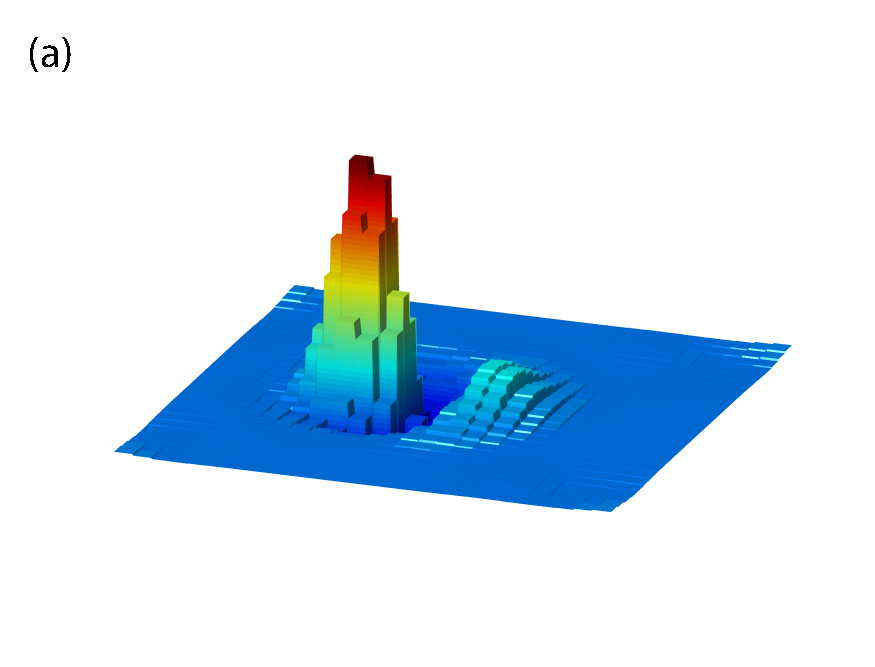
\includegraphics[height=.18\textheight]{images/27N_split_fourier.pdf}&
  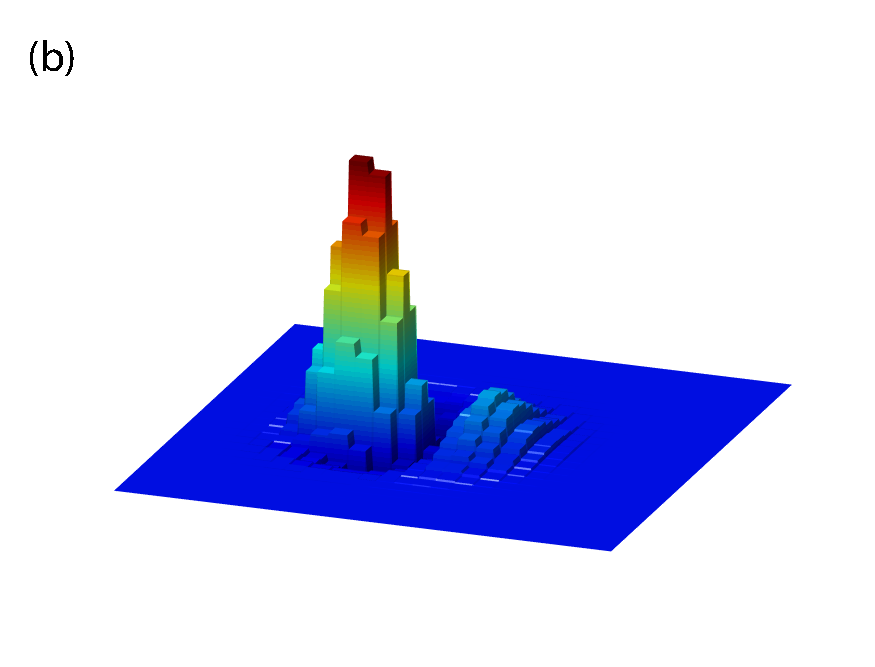
\includegraphics[height=.18\textheight]{images/27N_split_direct.pdf}&
  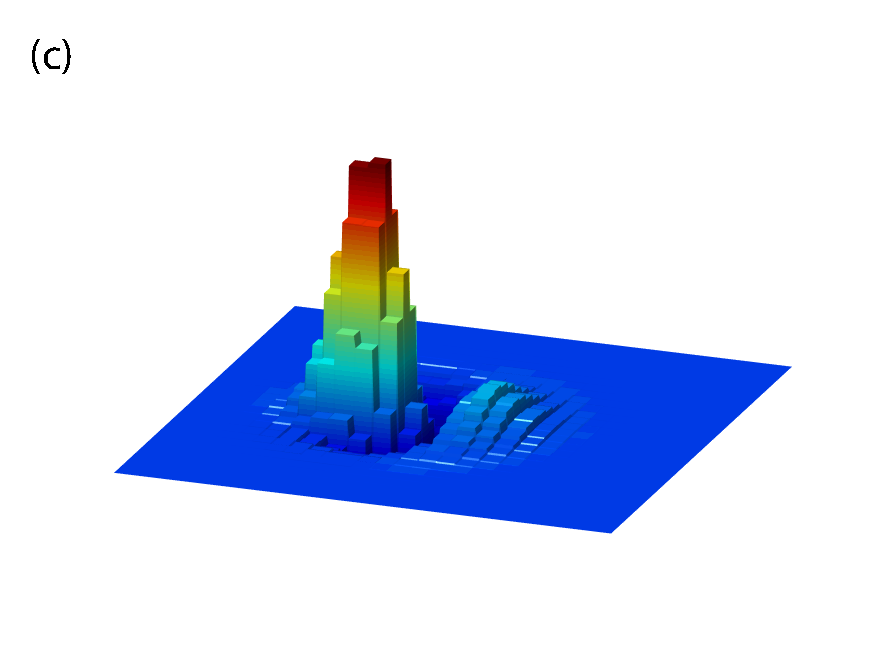
\includegraphics[height=.18\textheight]{images/27N_fourier.pdf}\\
  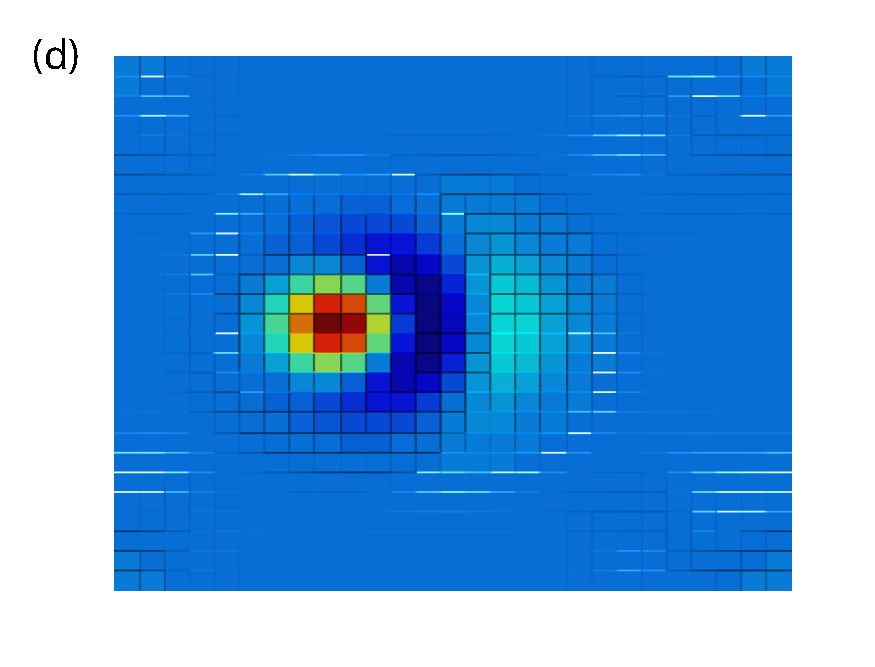
\includegraphics[height=.18\textheight]{images/27N_split_fourier_topdown.pdf}&
  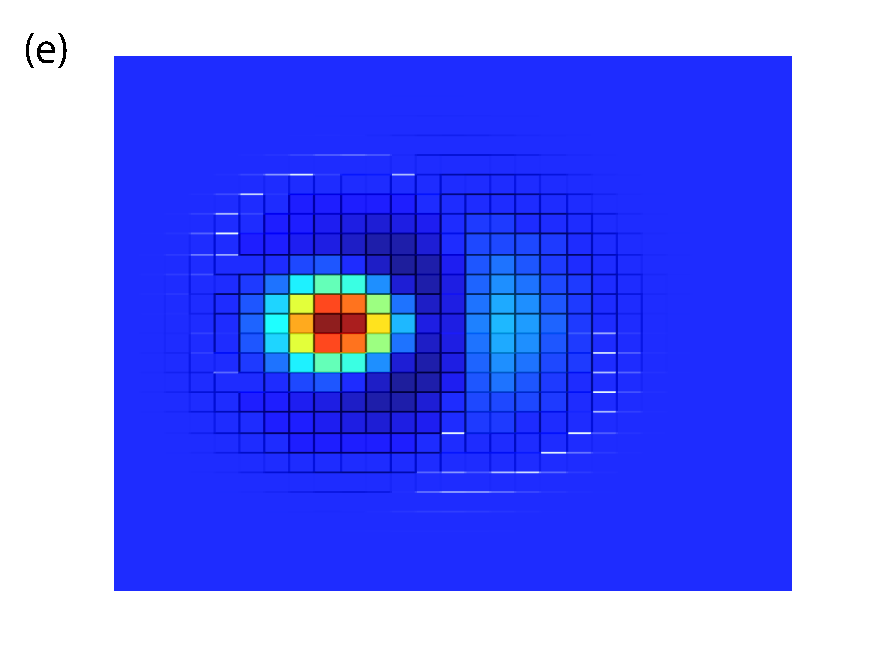
\includegraphics[height=.18\textheight]{images/27N_split_direct_topdown.pdf}&
  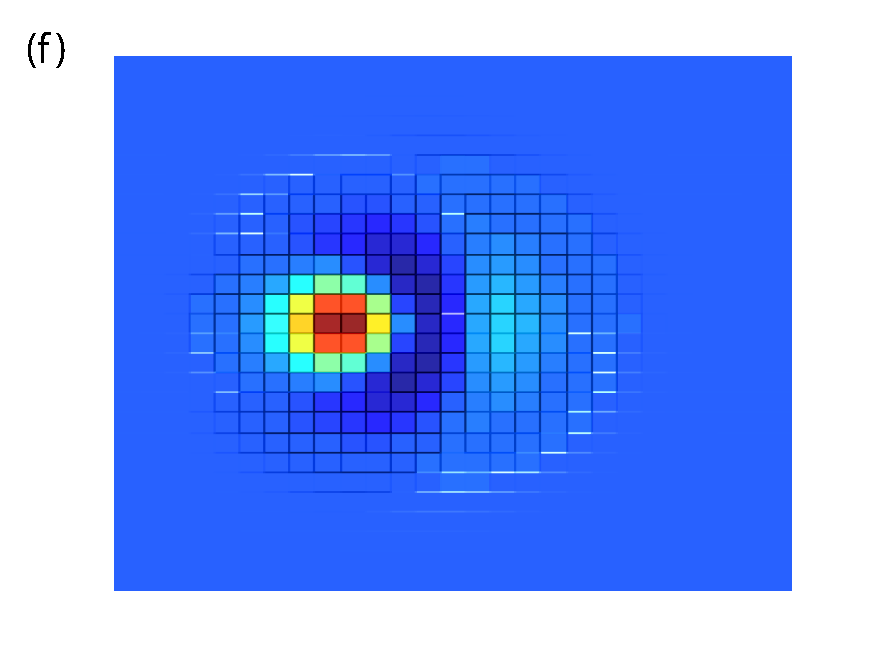
\includegraphics[height=.18\textheight]{images/27N_fourier_topdown.pdf}\\
\end{tabular}
\caption{\label{fig01} Evaluation of the collision operator using split and non-split forms: (a) and (d) the split form evaluated using the Fourier transform; (b) and (e) the split form evaluated directly; (c) and (f) the non-split form evaluated using the Fourier transform.}
\end{figure}
\end{center}

Another important issue that makes the non-split formulation more attractive is concerned 
with conservation of mass, momentum, and energy in the discrete solutions. It is the property of 
the exact Boltzmann collision operator that its mass, momentum, and temperature moments are zero. 
Generally, the conservation laws are satisfied only approximately when the Boltzmann equation is 
discretized. Many numerical approaches include mechanisms dedicated to enforcement of  
the conservation laws in discrete solutions in order to guarantee a physically meaningful result.

 \begin{table}[h]
  \begin{tabular}[c]{ c c c c c | c c c c }
  \hline
  \multicolumn{5}{c|}{Error in Conservation of Mass} &
  \multicolumn{4}{c}{Error in Conservation of Temperature}\\
    \hline 
    & \multicolumn{2}{c|}{Split} & \multicolumn{2}{c|}{Non-split} &
    \multicolumn{2}{c|}{Split} & \multicolumn{2}{c}{Non-split} \\
    \hline
    $n$ & Fourier& Direct & Fourier & Direct 
        & Fourier& Direct & Fourier & Direct \\
    \hline
    9   & 0.37 & 1.26 & 1.71E-5 & 1.92E-5 &
          3.51 & 1.69 & 1.71E-2 & 1.84E-2  \\
    15  & 0.10 & 1.20 & 1.45E-5 & 1.71E-5 & 
          0.29 & 1.25 & 1.64E-3 & 3.15E-3 \\
    21  & 0.18 & 1.18 & 0.67E-5 & 0.93E-5 & 
          1.38 & 1.24 & 5.61E-5 & 1.75E-3 \\
    27  & 0.18 & 1.18 & 0.61E-5 & 0.86E-5 & 
          1.37 & 1.24 & 5.40E-4 & 1.05E-3 \\
    \hline
  \end{tabular}
\caption{\label{tab02} Absolute errors in conservation of mass and temperature in the discrete collision integral computed using split and non-split formulations.}
\end{table}

It was observed that if no measures are introduced to enforce the conservation laws,  
solutions to the problem of spatially homogeneous relaxation obtained using the 
split formulation of the collision integral exhibit large, on the order of 5\%\ errors in 
temperature. The mass and momentum are also poorly conserved in this case. 
At the same time, solutions obtained using the non-split formulation had their mass, momentum,
and temperature accurate to three or more digits. To further explore this phenomena, 
we evaluated the collision operator in both split and non-split forms and computed its mass, 
momentum, and temperature moments. The solution was taken to be the sum of two Maxwellians 
in the example above. The numbers of velocity cells were 
varied from 9 to 27. In both split and non-split 
formulations of the collision integral, the decomposed form (\ref{eq:I_decomp_continuous}) of the solution was 
used. For both forms, evaluation of the collision operator was done directly and using the Fourier transform. 
The results are summarized in Table~\ref{tab02}. It can be seen that errors in the mass and 
temperature in the non-split formulation are several orders of magnitude smaller than in 
the split formulation. The errors are also larger in the case of direct evaluation. 
A possible explanation to this is the combined effect of finite precision 
arithmetic and truncation errors in integration that lead to catastrophic cancellation 
when gain and loss terms are combined. 
We note that in 
both split and non-split forms, fulfilment of 
conservation laws requires exact cancellation of the respective integration 
sums. 
When the gain and
loss terms are computed separately using numerical quadratures, the 
relative truncation errors are expected to be acceptable for each of the terms. 
This may change, however, when the terms are combined. It is 
conceivable that significant digits cancel in the two terms and the 
truncation errors are promoted into significance, manifesting in strong 
violations of conservation laws. At the same time, increasing 
the number of velocity cells may not remedy the problem 
due to the expected accumulation of roundoff 
errors. Indeed, evaluation of the gain term in (\ref{eq:I_split}) requires 
$O(M^8)$ arithmetic operations. 
It is possible that combination of large and small values in the finite 
precision arithmetic results in loss of low order digits and a significant 
accumulation of roundoff. When the gain and loss terms are combined, 
this, again, will lead to loss of significance and to perturbations of 
conservation laws. In the case when both the  
non-split form and the decomposition (\ref{eq:I_decomp_continuous}) are used, 
much of the cancellation is happening 
on the level of the integrand. 
We hypothesize here 
that the resulting values of the integrand are smaller and vary less 
in scale. As a result, the accumulated absolute truncation and 
roundoff errors are also smaller, which gives better accuracy in 
conservation laws.

Because of the poor conservation properties and because of the 
susceptibility to aliasing errors we do not recommend the 
split form (\ref{eq:I_split}) for numerical implementation. 


\section{0d Homogeneuous Relaxation}

In this section we present results of solution of the problem of 
spatially homogeneous relaxation using Fourier evaluation of the 
collision operator. Two cases of initial data were considered. In 
both cases, the initial data is a sum of two Maxwellian densities. 
In the first case, the 
dimensionless densities, bulk velocities, and temperatures of the 
Maxwellians are $n_1=1.0007$, $n_2=2.9992$, 
$\bar{\vec{u}}_{1}=(1.2247,0,0)$, $\bar{\vec{u}}_{2}=(0.4082,0,0)$,
$T_{1}=0.2$, $T_{2}=0.7333$. These parameters correspond to upstream 
and downstream conditions of the Mach 3 normal shock wave.  
In the second case, we use the parameters of the example of the previous  
section: $n_{1}=1.6094$, $n_{2}=2.8628$, $\bar{\vec{u}}_{1}=(0.7750,0,0)$, $\bar{\vec{u}}_{2}=(0.4357,0,0)$, $T_{1}=0.3$, and $T_{2}=0.464$. These 
parameters correspond to upstream and downstream conditions of a Mach 1.55 
shock wave. 

In Figures~{\ref{fig02}} and {\ref{fig03}}, relaxation of moments in the 
Mach~3.0 and Mach~1.55 solutions are presented. In the case of Mach~3.0, 
$M=33$ velocity cells were used in each velocity dimension with one 
velocity node on each cell, $s=1$. In the case of Mach~1.55, $M=15$ and $s=1$ 
were used. In the computed solutions, the collision operator was evaluated 
both using the Fourier transform and directly. In the Mach 3.0 instance, the directional 
temperature moments were compared to the moments obtained from a DSMC solution
\cite{Boyd1991411}. 

\begin{center}
\begin{figure}[h]
\centering
  \begin{tabular}{@{}cc@{}}
  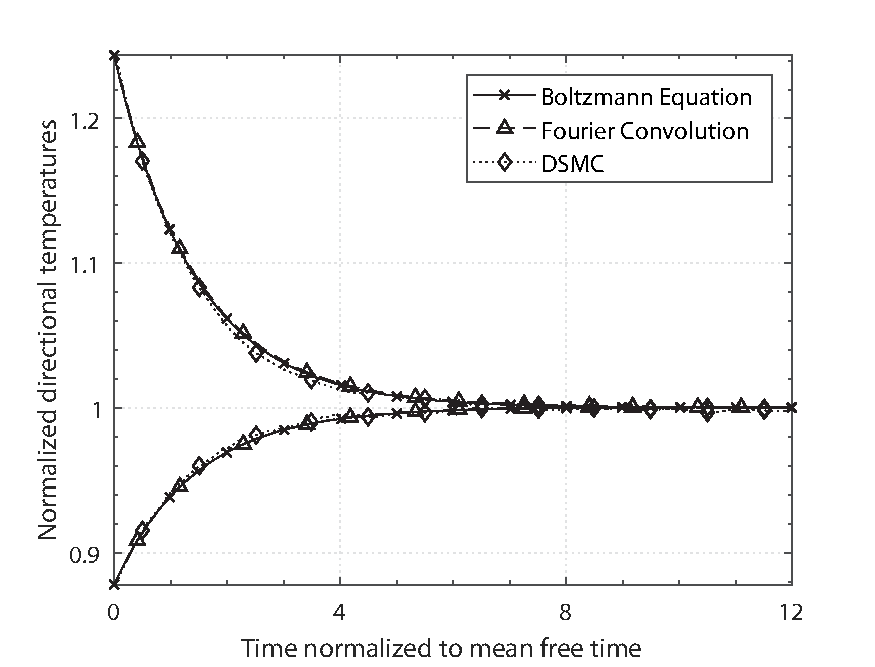
\includegraphics[height=.218\textheight]{images/m300_N33_mom2.pdf}&
  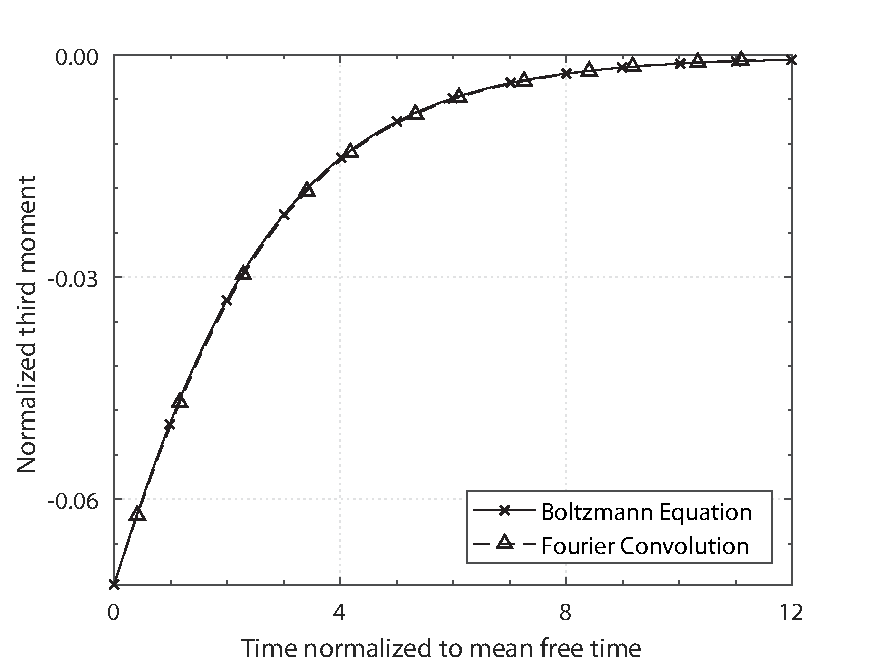
\includegraphics[height=.218\textheight]{images/m300_N33_mom3.pdf}\\      
  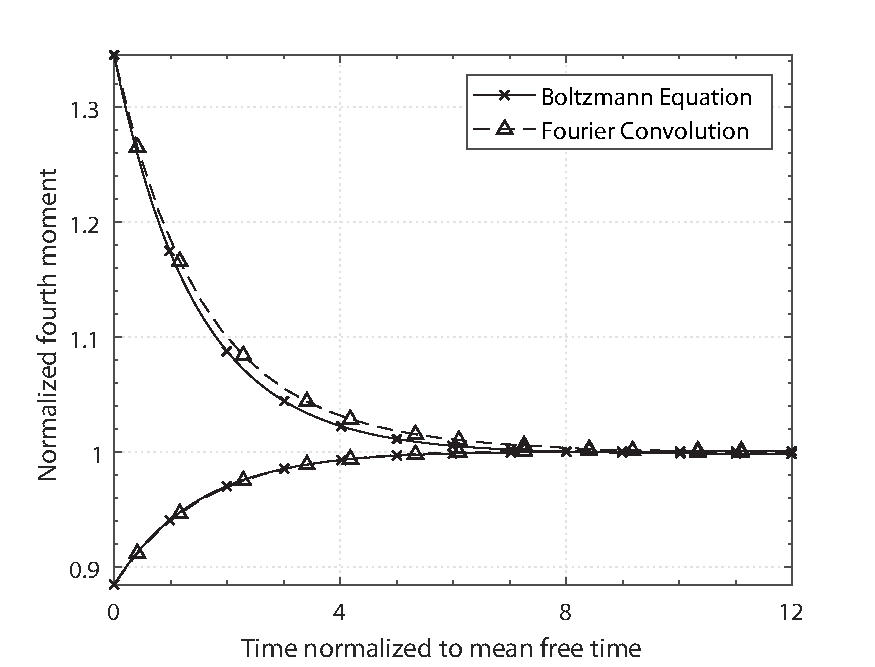
\includegraphics[height=.218\textheight]{images/m300_N33_mom4.pdf}&
  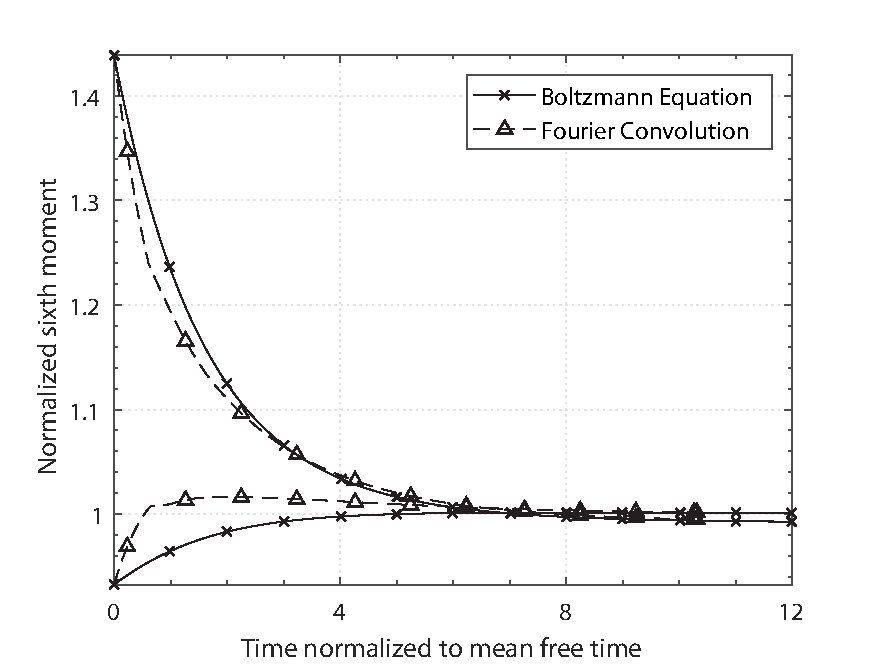
\includegraphics[height=.218\textheight]{images/m300_N33_mom6.pdf}\\
  \end{tabular}
\caption{\label{fig02} Relaxation of moments $f_{\varphi_{i,p}} = 
\int_{R^3} (u_{i}-\bar{u}_{i})^p f(t,\vec{u})\, du$, $i=1,2$, $p=2,3,4,6$ 
in a mix of Maxwellian streams corresponding to a shock wave with 
Mach number 3.0 obtained by solving the Boltzmann equation using Fourier and direct evaluations of the collision integral. In the case of $p=2$, the relaxation of moments 
is also compared to moments of a DSMC solution \cite{Boyd1991411}. }
\end{figure}
\end{center}

\begin{center}
\begin{figure}[h]
\centering
  \begin{tabular}{@{}cc@{}}
  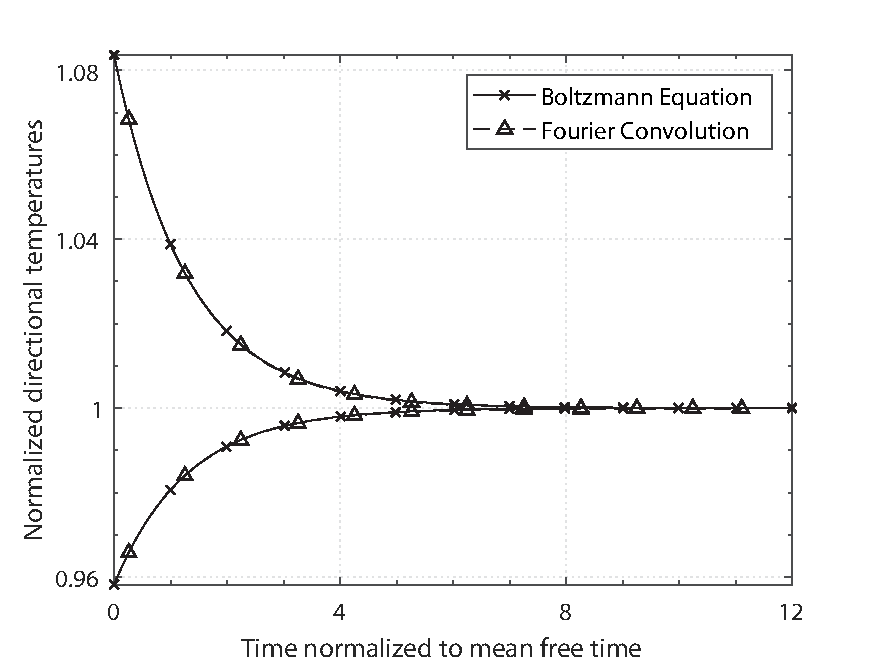
\includegraphics[height=.218\textheight]{images/m155_15N_mom2.pdf}&
  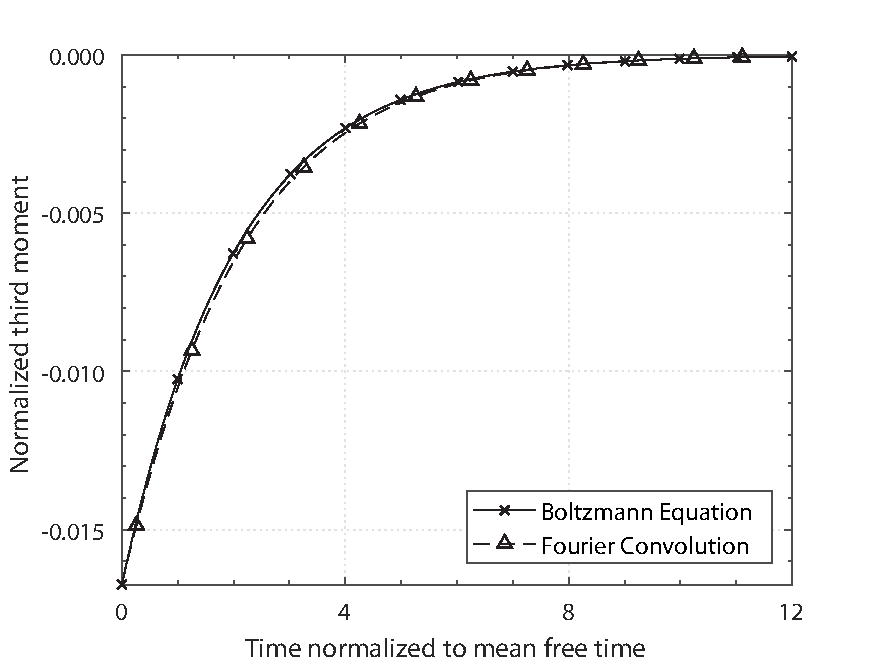
\includegraphics[height=.218\textheight]{images/m155_15N_mom3.pdf}\\      
  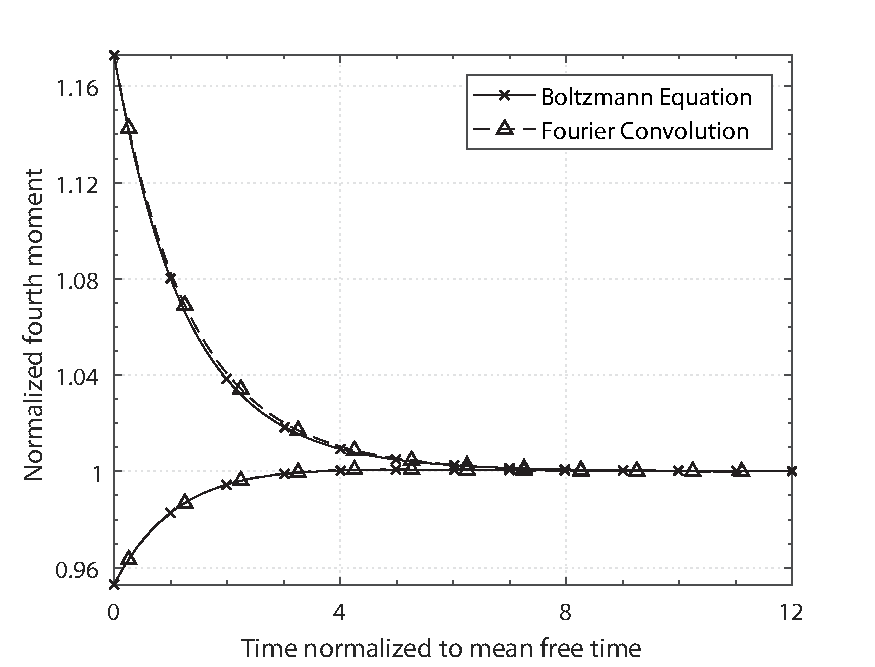
\includegraphics[height=.218\textheight]{images/m155_15N_mom4.pdf}&
  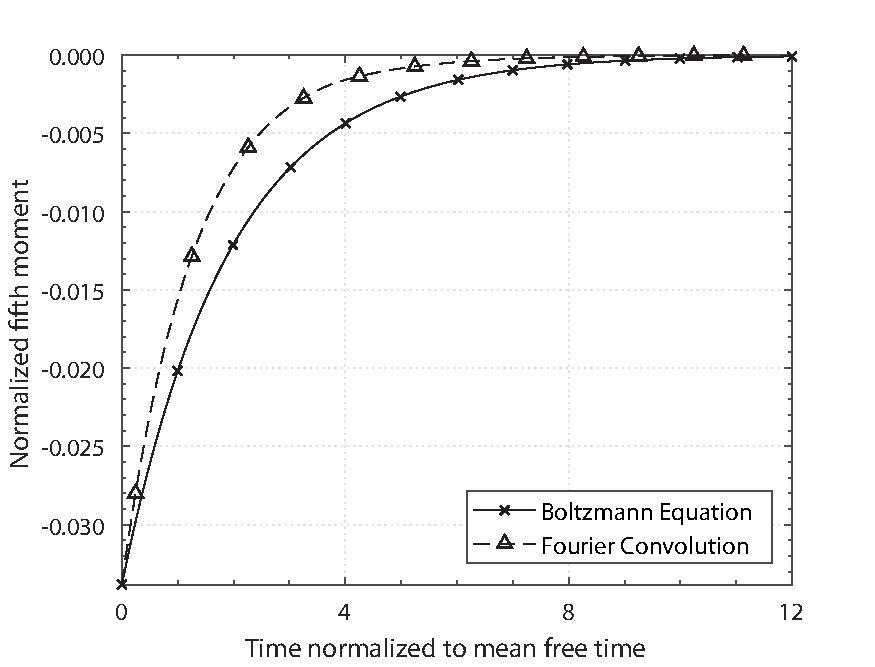
\includegraphics[height=.218\textheight]{images/m155_15N_mom6.pdf}\\
  \end{tabular}
\caption{\label{fig03} Relaxation of moments $f_{\varphi_{i,p}}$, $i=1,2$, $p=2,3,4,6$ 
in a mix of Maxwellian streams corresponding to a shock wave with 
Mach number 1.55 obtained by solving the Boltzmann equation using Fourier and direct evaluations of the collision integral.}
\end{figure}
\end{center}

It can be seen that the solutions obtained by the Fourier evaluation of the collision 
integral are close to those computed by the direct evaluation. The low order moments 
are in excellent agreement for both presented solutions. However, there are 
differences in the higher moments. It appears that the differences are caused 
by a small amount of the aliasing error in the solutions. This can be reduced 
by padding the solution and the kernel with zeros at the expense of higher numerical 
costs, both in time and memory. Overall, however, the $O(M^6)$ evaluation of 
the collision operator using the Fourier transform appears to be consistent 
and stable. 

It can be seen in Figure \ref{fig02} that the higher moments suffer more error than the lower moments.
It can be seen that the fourth moment has modest divergences from the direct evaluation, while the sixth moment diverges greatly in the direct evaluation.
This author believes that this due to the fact that we have more aliasing towards the ends of the domain. 
The higher moments will give much more weight to those parts of the domain than earlier moments. 
Indeed, Figure \ref{fig01} supports this hypothesis as we can see the edges of the domain had gain mass.

\section{Zero-Padding}

As discussed in section \ref{sec:lin_conv_fin_seq}, we saw that it is possible to reduce the amount of error from the calculations if we zero-pad the resulting sequence. These results show how zero-padding affects the error of the method as a function of the number of zeros that are added to the sequence. 

In section \ref{sec:lin_conv_fin_seq}, we showed that if want to completely eliminate any aliasing effect, then we must pad $f$ to length $2M - 1$ completely remove any aliasing effects from taking the inverse DFT to retrieve back $I_j$. However, this is prohibitive since that would mean adding $\mathcal{O}(M^6)$ zeros to $A$ in order to remove any aliasing effects from $\calF[A]$. Since we need to double its length in each dimension, that results in a 64 times increase in the memory storage of $\calF[A]$. 
As discussed in section \ref{sec:periodic_cont}, we assume that the shape of the function helps with the zero-padding and argue that we need only modest zero-padding to eliminate aliasing error.
However, we can combine modest zero padding with the fact that $f$ approaches zero in the edges of the domain to remove the numerical effects of aliasing rather quickly.

Zero-padding was accomplished by adding $n_{\text{pad}}$ zeros to each side of the sequence of $f$. Note that since $f$ is 3-dimensional, this means that symmetrically padding $f$ with $n_{\text{pad}}$ zeros on each size results in a size increase of $8n_{\text{pad}}^3$ (where the 8 comes from the fact that we are symmetrically padding) in the amount of numbers that must be stored. In addition, to naively perform the calculations, we must also zero-pad the $A$ kernel. This results in a memory increase of $64n_{\text{pad}}^6$. This of course then becomes restrictive as the number zeros increases since we will then run out of memory rather quickly. However, as the table below shows, even a modest increase in the number of zeros results in much lower error compared to the the straight-forward method presented earlier.

Table \ref{tab:padding_m155} shows how zero padding affected the accuracy of the method compared to a direct evaluation. These results were gathered using the parameters: $n_{1}=1.6094$, $n_{2}=2.8628$, $\bar{\vec{u}}_{1}=(0.7750,0,0)$, $\bar{\vec{u}}_{2}=(0.4357,0,0)$, $T_{1}=0.3$, and $T_{2}=0.464$ which corresponds to a mach 1.55 simulation. The table shows the error between the DFT method and direct method by symmetrically padding by zeros. Note that $n_{\text{pad}} = 1$ means that two 0s were added, one 0 to both ends of the sequence.

 \begin{table}[h]
  \begin{tabular}[c]{ c c c | c c | c c }
  \hline
  \multicolumn{1}{c}{} &
  \multicolumn{2}{c|}{$N = 9$} &
  \multicolumn{2}{c|}{$N = 15$} &
  \multicolumn{2}{c}{$N = 21$} \\
    \hline 
    $n_{\text{pad}}$ & $L_{\max}$  & $L_1$ & $L_{\max}$  & $L_1$ & $L_{\max}$  & $L_1$\\
    \hline
0 & 4.93E-05 & 3.74E-04 & 6.08E-05 & 4.66E-04 & 8.51E-05 & 5.39E-04\\
1 & 5.19E-07 & 1.15E-06 & 2.61E-07 & 1.33E-06 & 1.18E-06 & 8.79E-06\\
2 & 5.19E-07 & 1.14E-06 & 2.61E-07 & 2.93E-07 & 8.73E-08 & 9.59E-08\\
3 & 5.19E-07 & 1.14E-06 & 2.61E-07 & 2.93E-07 & 7.33E-09 & 9.59E-08\\
4 & 5.19E-07 & 1.14E-06 & 2.61E-07 & 2.93E-07 & 8.73E-08 & 9.58E-08\\
    \hline
  \end{tabular}
\caption{\label{tab:padding_m155} The $L_{\max}$ and $L_1$ errors as we increase $n_{\text{pad}}$. }
\end{table}

The table shows that the zero-padding the method results in more accuracy in the method. Remarkably, very little zero-padding must be done for the method to converge in accuracy. For both $N=9$ and $N=15$, the method converges in accuracy after symmetrically padding by two zeros. $N=21$ converged after $n_{\text{pad}} = 3$. 
These results suggest that the assumption of $f$ approaching zero rapidly in the edges of the domain is a valid one since not many zeros are needed to reach a convergence in accuracy. In addition, the author performed padding up to $n_pad{\text{pad}}=8$  for the $N=15$ case without seeing any substantial change from the above $n_{\text{pad}}=4$ case (and therefore omitted from the above table). This of course is much beyond the required $M-2$ zeros needed to achieve perfect accuracy, so any remaining error is an artifact of numerics.

However, padding by zeros will have an impact on the performance of the method as we increase the number of operations required to fully complete the calculations. The table below shows the amount of seconds the DFT along with how long the direct method took without padding.

 \begin{table}[h]
  \begin{tabular}[c]{ c c c | c c | c c }
  \hline
  \multicolumn{1}{c}{} &
  \multicolumn{2}{c|}{$N = 9$} &
  \multicolumn{2}{c|}{$N = 15$} &
  \multicolumn{2}{c}{$N = 21$} \\
    \hline 
    $n_{\text{pad}}$ & time (s)  & speed up & time (s)  & speed up & time (s)  & speed up\\
    \hline
0 & 0.22 & 6.28 & 1.18 & 40.38 & 6.09 & 114.30\\ 
1 & 0.19 & 7.27 & 1.65 & 28.95 & 11.18 & 62.27\\ 
2 & 0.31 & 4.36 & 6.23 & 7.66 & 33.19 & 20.97\\ 
3 & 0.97 & 1.41 & 6.30 & 7.58 & 33.10 & 21.03\\ 
4 & 2.13 & 0.64 & 11.40 & 4.19 & 51.07 & 13.63\\ 
  
    \hline
  \end{tabular}
\caption{\label{tab:timing_padding_m155}  How performance of the method decreases as we increase $n_{\text{pad}}$.}
\end{table}

As we can see from the table, the the fourier method still outperforms the direct method in time. However, the speed up drops dramatically as more zeros are added. In the $N=21$, the speed was reduced by half by adding one zero in each dimension, showing a increased time complexity cost for the increase in accuracy. 
In the $N=21$, the speed up drops by a third on $n_{\text{pad}} = 2$ to 20.97. However, zero-padding gives a degree of flexibility to the method to balance time and accuracy.

\section{The Model Kinetic Equations and the Rel-ES Method}


\subsection{The BGK Model}
\label{eq:coll_bgk_sec}
One of the difficulties with dealing with the Boltzmann equation is that it depends on the product of two distribution functions \cite{Kremer2010}, where
\begin{equation}
I[f] = \int(f_1' f' - f_1 f) g\, b \, db\, d\varepsilon\, d\vecv\, .
\end{equation}
We drop the integral limits for simplicity. We aim to simplify the structure of the collision term while maintaining the same basic properties. One such method was formulated by Bhatnagar, Gross, and Krook which is known as the BGK model \cite{BGK54}. From Strutchup \cite{Struchtrup2005}, we start by assuming that the post collision terms are close to Maxwellian, that is $f_1' \approx f_{M_1}'$ and $f' \approx f'_{M}$. We rewrite (\ref{eq:coll_bgk_sec}) as
\begin{equation}
\label{eq:bgk_step1}
\int  f_{M_1}' f'_{M} - f f_1 g\, b \, db\, d\varepsilon\, d\vecv\, .
\end{equation}
$\ln f_M$ is a linear combination of the collision invariants, so we have that $f_{M_1}' f'_{M}=f_{M_1} f_{M}$. We can then rewrite (\ref{eq:step1}) as 
\begin{equation}
\label{eq:bgk_step2}
f_M \int f_{M_1} g\, b \, db\, d\varepsilon\, d\vecv\, - f \int f_1 g\, b \, db\, d\varepsilon\, d\vecv\, .
\end{equation}
Lastly, we assume that the difference between the two integrals may be neglected. This leads to the BGK collision term
\begin{equation}
\label{eq:bgk}
\Psi_{\text{bgk}} = -\nu(f-f_M)\, 
\end{equation}
where
\begin{equation}
\nu = \int f_1 g\, b \, db\, d\varepsilon\, d\vecv\, .
\end{equation}
We refer to (\ref{eq:bgk}) as the BGK collision operator. If $\nu$ is known, then the BGK collision operator can be computed fast. However, since $\nu$ is not always known during execution time, it is sometimes easier to calculate $\nu$ as
\begin{equation}
\nu = \frac{P}{\mu}
\end{equation}
where $P$ is pressure and $\mu$ is the dynamic viscosity.

An important property of the BGK collision integral is that it conserves the first three moments, that is
\begin{equation}
\label{eq:bgk_conservative}
\begin{split}
	\int_{\mathbb{R}^3}  \Psi_{\text{bgk}}(t,\vec{x},\vec{v}) d\vec{v} = 0\, , & \\
	\int_{\mathbb{R}^3} v_i \Psi_{\text{bgk}}(t,\vec{x},\vec{v}) d\vec{v} = 0\, , & \quad i=1,2,3  \\
	\int_{\mathbb{R}^3} C^2 \Psi_{\text{bgk}}(t,\vec{x},\vec{v}) d\vec{v} = 0 \, .&
\end{split}
\end{equation}

\subsection{The ES-BGK Model}
Calculation of the Prandtl number from the BGK model leads to a Prandtl number of 1 \cite{Struchtrup2005}. In order to recitfy this, Holway \cite{H66} proposed the ellipsoidal statistical BGK model, known as the ES-BGK model. In the ES-BGK model, the Maxwellian is replaced by an anisotropic Gaussian.

First define $\vec{c} = \vecv - \bar{\vecv}$. Next, we define the stress tensor, $\Theta$, a $3 \times 3$ matrix such that
\begin{equation}
\Theta_{ij} = \frac{1}{n} \int_{\R^3} c_i c_j f d\vecv \, .
\end{equation}
We also define $\T = (1-\alpha)RTI-\alpha \Theta$ where $T$ is the temperature and $I$ is the $3 \times 3$ identity matrix. $\alpha$ is an adjustment factor used to adjust the Prandtl number of the equation,
\begin{equation}
Pr = \frac{1}{1-\alpha} \, .
\end{equation}
$\alpha$ must also be chosen such that $\T$ is symmetric positive definite (SPD). Zheng \cite{ZhengY2004} showed that $\alpha \in [-1/2,1)$ was sufficient to ensure SPD. We define the ESBGK collision operator as 
\begin{equation}
\label{eq:esbgk}
\Psi_{\text{ES}} = - \bar{\nu}(f-f_{\text{ES}})
\end{equation}
where
\begin{equation}
f_{\text{ES}}(\vecv) = \frac{n}{(\pi^3 \det(2\T))^{1/2}} \exp(-\frac{\vec{c}^T \T^{-1} \vec{c}}{2}) \, .
\end{equation}

Next, we prove an important property of the ES-BGK for the Rel-ES model.

\begin{theorem}
Let $\T$ be SPD, then we have
\begin{equation}
\frac{1}{n} \int_{\R^3} \vec{c}\,\vec{c}^T f_{\text{ES}} \,  d\vec{c} = \frac{1}{n}\int_{\R^3} \vec{c}\,\vec{c}^T \frac{n}{(\pi^3 \det(2\T))^{1/2}} \exp(-\frac{\vec{c}^T \T^{-1} \vec{c}}{2}) = \T \, .
\end{equation}
\end{theorem}
\begin{proof}
We ignore the constants for now and drop them from the integral, so we are left with
\begin{equation}
\label{eq:no_consts}
{\cal J}= \int_{\R^3} \vec{c} \, \vec{c}^T \exp(-\frac{\vec{c}^T \T^{-1} \vec{c}}{2}) \, .
\end{equation}
Since $\T$ is SPD, we have that $\T = Q^T \Lambda Q$ for some orthogonal matrix $Q$ and diagonal matrix $\Lambda$. We perform change of variables $\vec{w} = Q\vec{c}$ on (\ref{eq:no_consts}). Since $Q$ is orthogonal, we have that $d\vec{w} = \det Q\, d \vec{c} =d\vec{c}$. Multiplying (\ref{eq:no_consts}) by $Q$ on the left and $Q^T$ on the right, (\ref{eq:no_consts}) becomes
\begin{equation}
\label{eq:change_of_var}
\int_{\R^3} \vec{w}\,\vec{w}^T \exp(-\frac{\vec{w}^T \Lambda^{-1} \vec{w}}{2}) d\vec{w}\, .
\end{equation}
We can see that (\ref{eq:change_of_var}) is 9 equations. Focusing on one equation in (\ref{eq:change_of_var}), we get
\begin{equation}
\label{eq:entries}
\int_{\R^3} w_i w_j \exp((-\lambda_1^{-1} w_1^2 - \lambda_2^{-1} w_2^2 - \lambda_3^{-1} w_3^2)/2) dw_1 dw_2 dw_3, \quad i,j=1,2,3.
\end{equation}
When $i \not = j$ we get that the above integral is zero since the function is an odd function centered around zero. Without loss of generality, fix $i=1$, $j=2$. We get 
\begin{equation*}
\int_{-\infty}^{\infty} w_1 e^{-\lambda_1^{-1}w_1^2/2} dw_1 \int_{-\infty}^{\infty} w_2 e^{-\lambda_2^{-1}w_2^2/2} dw_2 \int_{-\infty}^{\infty} e^{-\lambda_3^{-1}w_3^2/2} dw_3 .
\end{equation*}
We see that $\int_{-\infty}^{\infty} w_1 e^{-\lambda_iw_1^2/2} dw_1 = 0$ since it is an odd integral. 

If $i=j$ (again, without loss of generality, set $i=j=1$) in (\ref{eq:entries}), then we have that
\begin{align}
&\int_{-\infty}^{\infty} w_1^2 e^{-\lambda_1^{-1}w_1^2} dw_1 \int_{-\infty}^{\infty} e^{-\lambda_2^{-1}w_2^2} dw_2 \int_{-\infty}^{\infty} e^{-\lambda_3^{-1}w_3^2} dw_3 \nonumber \\
= &\left(\frac{2{\pi}}{\lambda_1^{-3}} \right)^{1/2} \left(\frac{2{\pi}}{{\lambda_2^{-1}}} \right)^{1/2} \left(\frac{2{\pi}}{{\lambda_3^{-1}}} \right)^{1/2} \nonumber\\
= & (2 \pi)^{3/2} \sqrt{\lambda_1 \lambda_2 \lambda_3} \lambda_1 \nonumber\\
= & (2 \pi)^{3/2} (\det \T)^{1/2} \lambda_1 \, ,
\end{align}
where we used that $\lambda_1 \lambda_2 \lambda_3 = \det \Lambda = \det T$. We now have that (\ref{eq:change_of_var}) can be written as
\begin{equation}
(2 \pi)^{3/2} (\det \T)^{1/2} \Lambda \, .
\end{equation}
Multiplying on the left by $Q^T$ on the left and $Q$ on the right to recover (\ref{eq:no_consts}), we get
\begin{align}
\cal{J} = & (2 \pi)^{3/2} (\det \T)^{1/2} Q^T \Lambda Q \nonumber\\
= & (2 \pi)^{3/2} (\det \T)^{1/2} \T \, .
\end{align}
We can now reintroduce the constants into (\ref{eq:no_consts}),
\begin{align*}
\frac{1}{n} \frac{n}{(\pi^3 \det(2\T))^{1/2}} \cal{J} &= \frac{1}{(\pi^3 \det(2\T))^{1/2}} \cal{J}\\
&= \frac{1}{(\pi^3 \det(2\T))^{1/2}} (2 \pi)^{3/2} (\det \T)^{1/2} \T \\
&= \T
\end{align*}
\end{proof}

\subsection{Rel-ES}

\subsection{Experimental Results: 0d Homogeneous Relaxation}

In this section we present results of solution of the problem of 
spatially homogeneous relaxation using Fourier evaluation of the 
collision operator. Two cases of initial data were considered. In 
both cases, the initial data is a sum of two Maxwellian densities. 
In the first case, the 
dimensionless densities, bulk velocities, and temperatures of the 
Maxwellians are $n_1=1.0007$, $n_2=2.9992$, 
$\bar{\vec{u}}_{1}=(1.2247,0,0)$, $\bar{\vec{u}}_{2}=(0.4082,0,0)$,
$T_{1}=0.2$, $T_{2}=0.7333$. These parameters correspond to upstream 
and downstream conditions of the Mach 3 normal shock wave.  
In the second case, we use the parameters of the example of the previous  
section: $n_{1}=1.6094$, $n_{2}=2.8628$, $\bar{\vec{u}}_{1}=(0.7750,0,0)$, $\bar{\vec{u}}_{2}=(0.4357,0,0)$, $T_{1}=0.3$, and $T_{2}=0.464$. These 
parameters correspond to upstream and downstream conditions of a Mach 1.55 
shock wave. 

For evaluation of the shockwave, parameters $M=15$, $s=5$ were used to evaluate the shockwave. 

\begin{center}
\begin{figure}[h]
\centering
  \begin{tabular}{@{}cc@{}}
  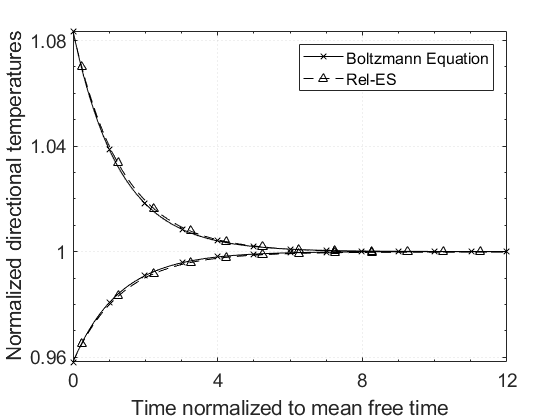
\includegraphics[height=.25\textheight]{images/reles_m155_5s15n_mom2.png}&
  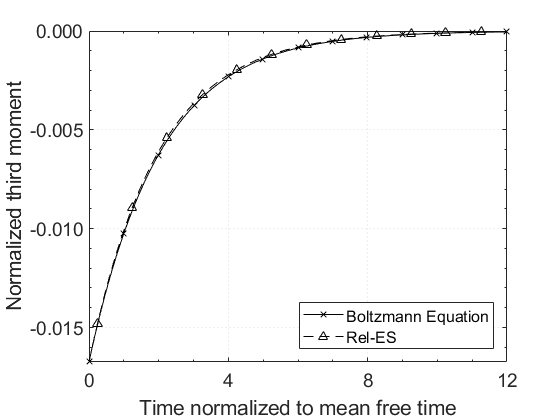
\includegraphics[height=.25\textheight]{images/reles_m155_5s15n_mom3.png}\\      
  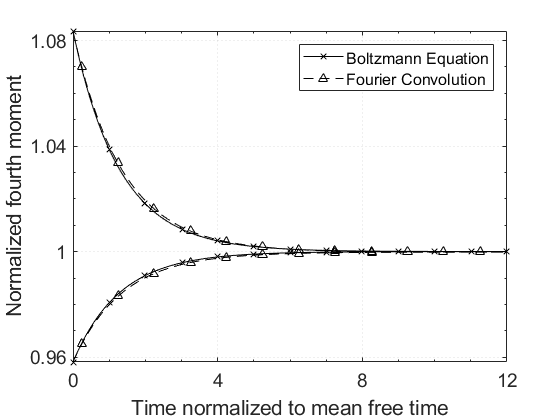
\includegraphics[height=.25\textheight]{images/reles_m155_5s15n_mom4.png}&
  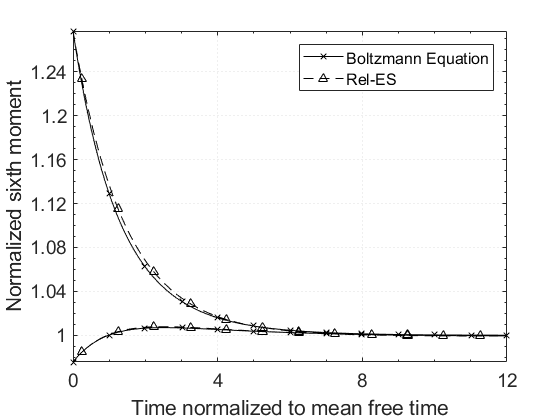
\includegraphics[height=.25\textheight]{images/reles_m155_5s15n_mom6.png}\\
  \end{tabular}
\caption{\label{fig03} Relaxation of moments $f_{\varphi_{i,p}}$, $i=1,2$, $p=2,3,4,6$ 
in a mix of Maxwellian streams corresponding to a shock wave with 
Mach number 1.55 obtained by solving the Boltzmann equation using Fourier and direct evaluations of the collision integral.}
\end{figure}
\end{center}


\clearpage
\addcontentsline{toc}{chapter}{References}
\bibliographystyle{plain}
\bibliography{ffb10092017}
\end{document}